\documentclass[12pt]{article}
\usepackage[utf8]{inputenc}
\usepackage{amsmath}
\usepackage{systeme}
\usepackage{amsfonts}
\usepackage{graphicx}
\usepackage{enumitem}
\usepackage{hyperref}
\usepackage{xcolor}
\usepackage{kbordermatrix}
\usepackage{centernot}
\usepackage{xcolor}
\usepackage{amsmath,amssymb,amsthm}
\usepackage{algorithmic}

\title{%
	\textbf{Notițe Seminar 12, 13}}

\begin{document}
	
	\maketitle
	
	\textbf{{Intro:}} În ultimele două seminarii vom face trecerea înspre algoritmul \textit{Expectation Maximization} pentru mixturi de distribuții gaussiene (pe scurt, \textbf{EM/GMM}). Mixturile de distribuții gaussiene pot fi folosite pentru clusterizare (cu asignare \textbf{soft} a instanțelor la cluster, adică având o instanță,
	spunem că ea aparține tuturor clusterelor: cu probabilitatea $p_1$ aparține clusterului 1, cu probabilitatea $p_2$ aparține clusterului 2 etc.:). Cum anume? Vom vedea abia la finalul fișierului. Până atunci să țineți minte că toți pașii pe care îi facem sunt pentru a ajunge la o nouă modalitate de a clusteriza date din $\mathbb{R}$ (există EM/GMM pentru $\mathbb{R}^d$, dar nu avem timp să ajungem și acolo).
	
	Pe parcurs vom vedea de ce estimările în sensul verosimilității maxime (\textbf{MLE}) pe care le-ați aplicat în prima parte a semestrului sunt valide. Mai mult, vom da la un moment dat și peste algoritmul \textbf{Bayes (Naiv) Gaussian} în varianta din notițele de la seminarul 7 în \textit{Privire de final Bayes Naiv}.
	
	\section{Remember/Intro}
	\subsection{Optimizare unidimensională}
	\subsubsection{Funcții de gradul 2}
	Fie $f:\mathbb{R} \rightarrow \mathbb{R}$, $f(x) = ax^2 + bx + c$, $a\neq 0$.
	\begin{itemize}
		\item Dacă $a>0$, atunci $f$ are minim, iar argumentul în care își atinge minimul este $x_\text{min} = \dfrac{-b}{2a}$
		\item Dacă $a<0$, atunci $f$ are maxim, iar argumentul în care își atinge maximul este $x_\text{max} = \dfrac{-b}{2a}$
	\end{itemize}
	\subsubsection{Orice funcții}
	Fie $f:\mathbb{R} \rightarrow \mathbb{R}$. Pentru a obține argumentul în care $f$ este maximizată/minimizată, putem urma pașii:
	\begin{itemize}
		\item calculăm derivata $f'(x)$
		\item rezolvăm ecuația $f'(x^*) = 0$ și-l obținem pe $x^*$.
		\item calculăm derivata a doua $f''(x)$
		\begin{itemize}
			\item dacă $f''(x) < 0, \forall x$, atunci $f$ este concavă, deci are maxim (global) și ne putem opri aici
			\item dacă $f''(x) > 0, \forall x$, atunci $f$ este convexă, deci are minim (global) și ne putem opri aici
			\item dacă $f''(x^*) < 0$, atunci $x^*$ este punct de maxim și ne putem opri aici
			\item dacă $f''(x^*) > 0$, atunci $x^*$ este punct de minim și ne putem opri aici
		\end{itemize}
	\end{itemize}
	\subsubsection{Trick}
	Cum $\ln$ este funcție crescătoare, avem că:
	$\arg\max_x f(x) = \arg \max \ln f(x)$.

	\subsection{ln}
	$$\ln(a\cdot b) = \ln a + \ln b$$
	$$\ln a^b = b\ln a$$
	\subsection{NA}
	NA vine de la \textit{Not Available}. Dacă într-o matrice cu date avem o celulă fără valoare, vom introduce totuși valoarea NA.
	
	\subsection{Funcția indicator}
	Funcția \textbf{indicator}: $I : \{\text{True},\text{False}\} \rightarrow \{0,1\}$, $I(\text{True}) = 1$, $I(\text{False}) = 0$.
	
	În acest document voi folosi următoarea notație pentru funcția indicator: $1\{\text{True}\}=I(\text{True})=1$, $1\{\text{False}\}=I(\text{False})=0$.
	
	\subsection{PS}
	
	\subsubsection{Formule}
	Fie $X$, $Y$ două variabile aleatoare cu Val$(Y)=\{0,1\}$.
	
	\noindent \textbf{Formula de înmulțire/multiplicare}: 
	$$P(X=x,Y=y) = P(X=x)P(Y=y|X=x) = P(Y=y)P(X=x|Y=y)$$ 
	sau în notația pmf/pdf:
	$$p_{X,Y}(x,y) = p_X(x)p_{Y|X}(y|x) = p_Y(y)p_{X|Y}(x|y)$$
	
	\noindent \textbf{Formula probabilității totale/Probabilitatea marginală}
	$$P(X=x) = P(X=x,Y=0) + P(X=x,Y=1)$$
	sau în notația pmf/pdf:
	$$p_{X}(x) = p_{X,Y}(x,0)+p_{X,Y}(x,1)$$
	
	\noindent \textbf{Formula lui Bayes (FB)}
	$$P(Y=y|X=x) = \dfrac{P(X=x|Y=y)P(Y=y)}{P(X=x|Y=0)P(Y=0) + P(X=x|Y=1)P(Y=1)}$$
	sau în notația pmf/pdf:
	$$p_{Y|X}(y|x) = \dfrac{p_{X|Y}(x|y)p_Y(y)}{p_{X|Y}(x|0)p(0) + p_{X|Y}(x|1)p_Y(1)}$$
	
	\noindent\textbf{Media (E) unei variabile aleatoare discrete}
	
	$E[X] = \sum_{x \in \text{Val}(X)} x \cdot p_X(x)$
	
	Exemplu: $X:\begin{pmatrix}
	0 & 1\\
	0.1 & 0.9
	\end{pmatrix}$, $E[X] = 0 \cdot 0.1 + 1\cdot 0.9 = 0.9$.
	
	\subsubsection{Distribuții uzuale}
	\begin{itemize}
		\item 	Dacă $X \sim \text{Bernoulli}(\theta)$, atunci $X: \begin{pmatrix}
		0 & 1\\
		1-\theta & \theta
		\end{pmatrix}$. 
		
		$\theta$ este parametrul pentru \textbf{distribuția Bernoulli}. 
		
		Funcția masă de probabilitate (pmf) pentru X este 
		
		$p_X(x;\theta) = P(X = x;\theta) = \text{Bernoulli}(x;\theta) = \begin{cases}
		\theta & x = 1\\
		1-\theta & x=0
		\end{cases} =$
		
		$= \theta^x (1-\theta)^{1-x}.$
		
		Puteți verifica imediat ultimul ``='' de mai sus. Verificați-l!
		
		Uneori, $p_X$ este scris simplu ca $p$. 
		
		Uneori, partea ``;$\theta$" este înlocuită cu ``$|\theta$".
		
		Uneori, partea ``;$\theta$" este omisă. 
		
		\textbf{Exemplu}: $X: \begin{pmatrix}
		0 & 1\\
		0.3 & 0.7
		\end{pmatrix}$
		
		\textbf{Exemple de experimente aleatoare din spate}: aruncăm o monedă (care are probabilitatea $\theta$ să cadă H) și vedem dacă iese H sau T; aruncăm un zar cu 2 fețe (care are probabilitatea $\theta$ să cadă o față) și vedem ce față iese
		
		\item 	Dacă $X \sim \text{Categorială}(\pi_{v_1},\dots,\pi_{v_n})$, $\pi_{v_1}+\dots+\pi_{v_n} = 1$, atunci $X:\begin{pmatrix}
		v_1 & \dots & v_n\\
		\pi_{v_1} & \dots & \pi_{v_n}
		\end{pmatrix}$. 
		
		$\pi_{v_1},\dots,\pi_{v_n}$ sunt parametrii pentru \textbf{distribuția Categorială}. 
		
		Funcția masă de probabilitate (pmf) pentru X este 
		
		$p_X(x;\pi_{v_1},\dots,\pi_{v_n}) = P(X = x;\pi_{v_1},\dots,\pi_{v_n}) = \text{Categorială}(x;\pi_{v_1},\dots,\pi_{v_n}) =$
		
		$=\begin{cases}
		\pi_{v_1} & x = v_1\\
		\pi_{v_2} & x = v_2 \\
		\vdots\\
		\pi_{v_n} & x = v_n
		\end{cases}=\pi_{v_1}^{1\{x=v_1\}} \pi_{v_2}^{1\{x=v_2\}} \dots \pi_{v_n}^{1\{x=v_n\}}$
		
		Puteți verifica imediat ultimul ``='' de mai sus. Verificați-l!
		
		Uneori, $p_X$ este scris simplu ca $p$. 
		
		Uneori, partea ``;$\pi_{v_1},\dots,\pi_{v_n}$" este înlocuită cu ``$|\pi_{v_1},\dots,\pi_{v_n}$".
		
		Uneori, partea ``;$\pi_{v_1},\dots,\pi_{v_n}$" este omisă.
		
		\textbf{Exemplu}: $X: \begin{pmatrix}
		1 & 2 & 3\\
		0.1 & 0.2 & 0.7
		\end{pmatrix}$
		
		\textbf{Exemplu de experiment aleator din spate}: aruncăm un zar cu $k$ fețe (probabilitatea să cadă fața $v_1$ este $\pi_{v_1}$ etc.) și vedem ce față iese
		
		\textbf{Observație}: Dacă X are doar două valori posibile, atunci distribuția Categorială este echivalentă cu distribuția Bernoulli dacă redefinim valorile posibile pentru Categorială să fie 0 și 1.
			
		\item Dacă $X \sim \mathcal{N}(\mu,\sigma^2)$, atunci funcția densitate de probabilitate (pdf) pentru X este
		
		$p_X(x;\mu,\sigma^2) = \mathcal{N}(x;\mu,\sigma^2) = \frac{1}{\sqrt{2\pi}\sigma} e^{-\frac{1}{2} (\frac{x-\mu}{\sigma})^2}$,
		
		iar $\mu,\sigma^2$ sunt parametrii pentru \textbf{distribuția normală/Gaussiană}. 
		
		Uneori, $p_X$ este scris simplu ca $p$. 
		
		Uneori, partea ``;$\mu,\sigma^2$" este înlocuită cu ``$|\mu,\sigma^2$".
		
		Uneori, partea ``;$\mu,\sigma^2$" este omisă. 
		
		\textbf{Exemplu}: $X \sim \mathcal{N}(\mu=2,\sigma^2=3^2)$:
		
		\begin{center}
			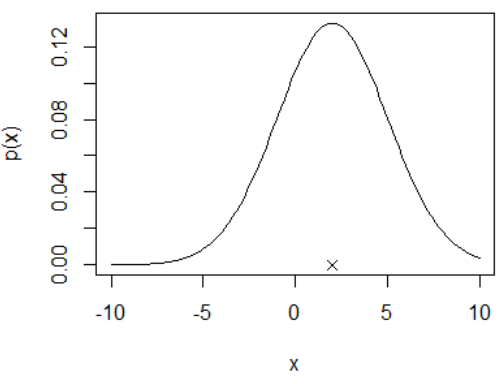
\includegraphics[width=0.75\linewidth]{screenshot001}
			
			(cu un ``x" a fost marcată media $\mu = 2$)
		\end{center}

		\textbf{Exemplu de experiment aleator din spate}: alegem un om și îi măsurăm înălțimea (presupunem că înălțimea urmează distribuția $\mathcal{N}(\mu,\sigma^2)$, de unde rezultă că e în jur de $\mu$ unități).
	\end{itemize}
	
	\subsubsection{2 formule folositoare pentru calculul $\mathcal{N}(x;\mu,\sigma^2)$ atunci când ne sunt furnizate valori pentru $\mathcal{N}(...;\mu=0,\sigma^2=1^2)$}
	$$\mathcal{N}(x;\mu,\sigma^2)=\frac{1}{\sigma}\mathcal{N}\left(\frac{x-\mu}{\sigma};0,1\right)$$
	$$\mathcal{N}(x;\mu=0,\sigma^2=1^2) = \mathcal{N}(-x;\mu=0,\sigma^2=1^2)$$
	Exemplu de aplicare:
	
	Știind că $\mathcal{N}(2;0,1)=0.053$, calculați $\mathcal{N}(1;9,4^2)$.
	
	$\mathcal{N}(1;9,4^2) = \frac{1}{4} \mathcal{N}(\frac{1-9}{4};0,1) = \frac{1}{4}\mathcal{N}(-2;0,1) = \frac{1}{4}\mathcal{N}(2;0,1) = \frac{0.053}{4} \approx 0.013$
	
	\noindent Observație: Dacă $X \sim \mathcal{N}(\mu,\sigma^2)$, atunci $Z=\dfrac{X-\mu}{\sigma} \sim \mathcal{N}(0,1)$. Transformarea $X\rightarrow Z = \dfrac{X-\mu}{\sigma}$ se numește \textbf{standardizare}.
	
	\subsubsection{VA iid}
	Fie $X_1, X_2, \dots, X_n$ variabile aleatoare independente și identic distribuite. Vom nota pe scurt acest lucru astel: $X_1, X_2, \dots, X_n$ - \textbf{VA iid}.
	
	$X_1, \dots, X_n$ - independente $\Rightarrow p_{X_1,\dots,X_n}(x_1,\dots,x_n) = p_{X_1}(x_1)\dots p_{X_n}(x_n)$
	
	$X_1, \dots, X_n$ - identic distribuite $\Rightarrow X_i \sim \text{Distribuție(parametri)},\forall i \in\{1,\dots,n\}$, adică există o singură distribuție cu o singură setare a parametrilor pe care o urmează fiecare $X_i$.
	
	\subsubsection{Mixturi de distribuții de probabilitate}
	
	Fie:
	\begin{itemize}
		\item un număr natural nenul $k$
		\item $k$ funcții pmf/pdf: $p^1(x;\theta_1), \dots, p^k(x;\theta_k)$, unde $\theta_1, \dots, \theta_k$ sunt parametri
		\item $k$ probabilități a căror sumă este 1: $\pi_1,\dots,\pi_k \in [0,1]$; $\pi_1+\dots+\pi_k=1$; aceste probabilități se numesc \textit{probabilități a priori de selecție}
	\end{itemize}
	
	\noindent Atunci următorul pmf/pdf reprezintă \textbf{mixtura celor $k$ distribuții sau pmf/pdf-uri}:
	$$p_X(x;\theta_1,\dots,\theta_k,\pi_1,\dots,\pi_k) = \pi_1 p^1(x;\theta_1) + \dots + \pi_k p^k(x;\theta_k)$$
	
	$\theta_1,\dots,\theta_k,\pi_1,\dots,\pi_k$ sunt parametrii pentru mixtura de distribuții de mai sus.
	
	Uneori, $p_X$ este scris simplu ca $p$. 
	
	Uneori, $p^i$ este scris simplu ca $p_i$. 
	
	Uneori, partea ``;$\theta_1,\dots,\theta_k,\pi_1,\dots,\pi_k$" este înlocuită cu ``$|\theta_1,\dots,\theta_k,\pi_1,\dots,\pi_k$".
	
	Uneori, partea ``;$\theta_1,\dots,\theta_k,\pi_1,\dots,\pi_k$" este omisă.
		
	Exemplu: 
	
	$p(x) = 0.2 \cdot \text{Bernoulli}(x;0.4) + 0.8\cdot\text{Bernoulli}(x;0.1)$
		
	$p(x) = 0.25\cdot \mathcal{N}(x;2,1^2) + 0.75\cdot\mathcal{N}(x;11,4^2)$ - \textbf{mixtură de gaussiene}
	
	\textbf{Completare la definiția pentru mixturi de distribuții probabiliste:}
	
	Considerăm următoarele presupuneri adevărate:
	
	$$Z \sim \text{Categorială}(\pi_1,\dots,\pi_k)$$
	$$(X|Z=j) \sim p_j(\theta_j)$$
	
	Atunci vom da chiar peste mixtura de distribuții definită mai sus: 
	\begin{align*}
	p_X(x) &\stackrel{\text{pb.marg.}}{=} p_{X,Z}(x,1)+\dots+p_{X,Z}(x,k) \\ 
	&\stackrel{\text{f.de înmulț.}}{=} p_Z(1) p_{X|Z}(x|1)+\dots+p_Z(k)p_{X|Z}(x|k) \\
	&= \pi_1 p_1(x) + \dots + \pi_k p_k(x)
	\end{align*}
	
	\textbf{Tricks utile mai târziu}: 
	
	$p_Z(j) = \pi_j = \pi_1^{1\{Z=j\}} \dots \pi_k^{1\{Z=j\}}$
	
	$p_{X|Z}(x|j) = p_j(x) = (p_1(x))^{1\{Z=j\}} \cdot \dots \cdot (p_k(x))^{1\{Z=j\}}$
	
	\textbf{Experimentul aleator din spate}: avem la dispoziție $k$ experimente; aruncăm un zar cu $k$ fețe care are distribuția Categorială dată de $\pi_1,\dots,\pi_k$ și în funcție de ce față a ieșit executăm experimentul corespunzător și vedem ce rezultat ne furnizează acel experiment; datele pe care le raportăm nu includ de obicei ce față a zarului a căzut
	
	\textbf{Exemplu de experiment aleator din spate} pentru $p(x) =0.25\cdot \mathcal{N}(x;2,1^2) + 0.75\cdot\mathcal{N}(x;11,4^2)$: aruncăm un zar cu 2 fețe (probabilitățile pentru fețe sunt 0.25 și 0.75); dacă a ieșit fața 1, atunci alegem un om din România și îi măsurăm înălțimea (presupunem că înălțimea unui român urmează distribuția $\mathcal{N}(2,1^2)$, de unde rezultă că e în jur de 2 unități); dacă a ieșit fața 2, atunci alegem un om din SUA și îi măsurăm înălțimea (presupunem că înălțimea unui american urmează distribuția $\mathcal{N}(11,4^2)$, de unde rezultă că e în jur de 11 unități); la final, raportăm doar înălțimea, să zicem 13 unități, fără să spunem ce față a zarului a ieșit.
	
	\textbf{Trei grafice} pentru $p(x) =0.25\cdot \mathcal{N}(x;2,1^2) + 0.75\cdot\mathcal{N}(x;11,4^2)$:
	
	(pe grafice, cu ``x" au fost marcate mediile $\mu = 2$ și $\mu = 11$)
	
	Graficul pentru $p(x)$:
	\begin{center}
		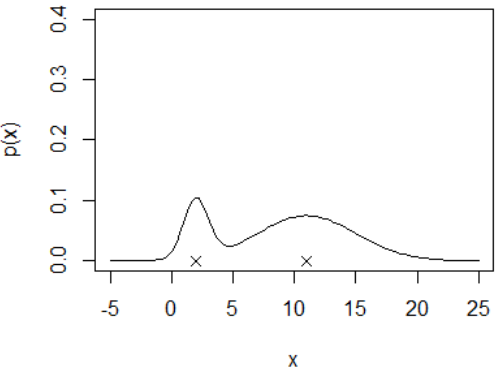
\includegraphics{screenshot002}
	\end{center}
	\newpage
	Graficul pentru $\mathcal{N}(x;2,1^2)$ și $\mathcal{N}(x;11,4^2)$:
	\begin{center}
		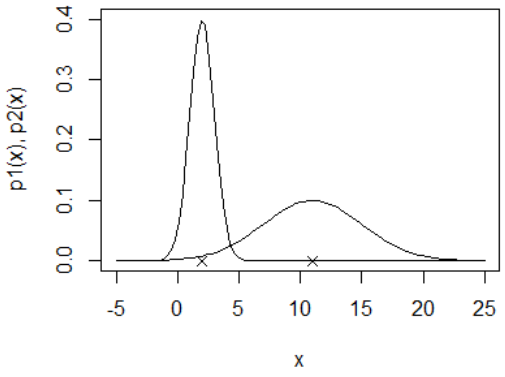
\includegraphics{screenshot003}
	\end{center}
	Graficul pentru $0.25 \cdot \mathcal{N}(x;2,1^2)$ și $0.75 \cdot \mathcal{N}(x;11,4^2)$:
	\begin{center}
		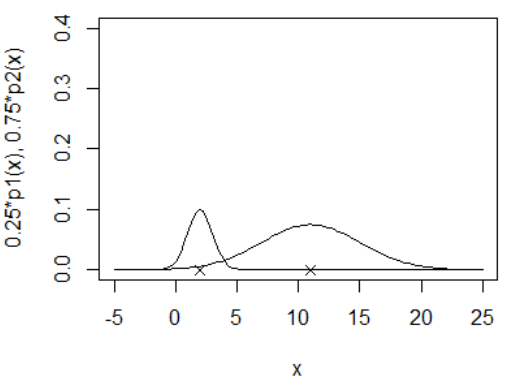
\includegraphics{screenshot004}
	\end{center}
	
	\subsubsection{MLE (vs MAP)}	
	
	În realitate, parametrii pentru distribuții nu sunt cunoscuți. În lumea reală avem date. Ca să ne putem \textit{juca} cu probabilități putem \textbf{estima} parametrii distribuțiilor de probabilitate din date. Modalitatea principală de estimare este cea în sensul verosimilității maxime (\textbf{MLE}). O alta este estimarea de probabilitate maximă a posteriori (MAP). În acest fișier vom folosi doar MLE.
	
	\noindent Fie $D$ datele pe care le observăm, iar $\theta$ parametrul pe care vrem să-l aflăm.
	
	$\theta_\text{MLE} = \arg \max_\theta \underbrace{p(D|\theta)}_{\text{funcția de verosimilitate/likelihood}}$
	
	($\theta_\text{MAP} = \arg \max_\theta p(\theta|D)$)
	
	\section{MLE}
	Pentru a ilustra conceptele de 
	\begin{itemize}
		\item \textbf{funcție de verosimilitate}
		\item \textbf{funcție de log-verosimilitate}
		\item \textbf{algoritm EM}
	\end{itemize}
	vom folosi 5 exerciții în care \textbf{tot timpul cerem să se maximizeze verosimilitatea datelor (observabile)}. Fiecare exercițiu vine cu ceva nou față de precedentele după cum se va vedea.
	
	Mai întâi vom da enunțurile exercițiilor, apoi le vom rezolva cu formule/algoritmi. În cele din urmă vom demonstra de ce formulele/algoritmii sunt așa cum sunt. Dacă un exercițiu are două subpuncte, vom deriva formulele/algoritmul doar pentru primul subpunct.
	
	\newpage
	
	\subsection{Exerciții}
	\subsubsection{Enunțuri}
	\begin{enumerate}
		\item \textbf{Exercițiul 1}
		
		Fie următorul set de date: D =
		\begin{tabular}{ |c|c|c| } 
			\hline
			X \\ 
			\hline
			0 \\ 
			0 \\ 
			0 \\
			1\\
			\hline
		\end{tabular}. 
	
	Presupunem următoarele:
	\begin{itemize}
		\item $X_1$, $X_2$, $X_3$, $X_4$ - VA iid: $X_i \sim \text{Bernoulli}(\theta)$
		\item $D=(x_1,x_2,x_3,x_4) = (0,0,0,1)$ - date/instanțe/observații generate de $X_1,X_2,X_3,X_4$.
	\end{itemize}
	Aflați parametrul $\theta_\text{MLE}$ care maximizează funcția de verosimilitate a datelor D.
		\item \textbf{Exercițiul 2}
		\begin{enumerate}
			\item 		Fie următorul set de date: D =
			\begin{tabular}{ |c|c|c| } 
				\hline
				X \\ 
				\hline
				1 \\ 
				2 \\ 
				3 \\
				\hline
			\end{tabular}. 
			
			Presupunem următoarele:
			\begin{itemize}
				\item $X_1$, $X_2$, $X_3$ - VA iid: $X_i \sim \mathcal{N}(\mu,\sigma^2=3^2)$
				\item $D=(x_1,x_2,x_3) = (1,2,3)$ - date/instanțe/observații generate de $X_1,X_2,X_3$.
			\end{itemize}
			Aflați parametrul $\mu_\text{MLE}$ care maximizează funcția de verosimilitate a datelor D.
			
			\item 	Fie următorul set de date: D =
			\begin{tabular}{ |c|c|c| } 
				\hline
				X \\ 
				\hline
				1 \\ 
				2 \\ 
				3 \\
				\hline
			\end{tabular}. 
			
			Presupunem următoarele:
			\begin{itemize}
				\item $X_1$, $X_2$, $X_3$ - VA iid: $X_i \sim \mathcal{N}(\mu,\sigma^2)$
				\item $D=(x_1,x_2,x_3) = (1,2,3)$ - date/instanțe/observații generate de $X_1,X_2,X_3$.
			\end{itemize}
			Aflați parametrii $\mu_\text{MLE}$, $\sigma^2_\text{MLE}$ care maximizează funcția de verosimilitate a datelor D.
		\end{enumerate}

		\item \textbf{Exercițiul 3}
		
		Fie următorul set de date:
		\begin{tabular}{ |c|c|c| } 
			\hline
			X \\ 
			\hline
			0 \\ 
			0 \\ 
			0 \\
			1\\
			NA\\
			\hline
		\end{tabular} $\rightarrow$ \begin{tabular}{ |c|c|c| } 
		\hline
		X \\ 
		\hline
		0 \\ 
		0 \\ 
		0 \\
		1\\
		$Z_1$\\
		\hline
	\end{tabular}. 
		
		Presupunem următoarele:
		\begin{itemize}
			\item $X_1$, $X_2$, $X_3$, $X_4$, $Z_1$ - VA iid: 
			\begin{itemize}
				\item $X_i \sim \text{Bernoulli}(\theta)$ - VA observabile
				\item $Z_1 \sim \text{Bernoulli}(\theta)$ - VA latente/ascunse/neobservabile
			\end{itemize}
			\item $D=(x_1,x_2,x_3,x_4) = (0,0,0,1)$ - date observabile/instanțe/observații generate de $X_1,X_2,X_3,X_4$.
			\item $D_l = (Z_1)$ - date latente/ascunse/neobservabile generate de $Z_1$ (puteam spune $D_l = (Z_2), Z_2\sim Z_1$ pentru a nu avea suprapunere de nume între data $Z_1$ și variabila $Z_1$, dar nu vrem să ne complicăm inutil)
			\item $D_c = (0,0,0,1,Z_1)$ - date complete generate de $X_1$, $X_2$, $X_3$, $X_4$, $Z_1$
		\end{itemize}
		Aflați parametrul $\theta_\text{MLE}$ care maximizează funcția de verosimilitate a datelor \textbf{D}.
		\item \textbf{Exercițiul 4} - algoritmul \textbf{Bayes (Naiv) Gaussian} în varianta din notițele de la seminarul 7 în \textit{Privire de final Bayes Naiv}
		
		\begin{enumerate}
			\item Fie următorul set de date: D =
			\begin{tabular}{ |c|c|c| } 
				\hline
				X & Y \\ 
				\hline
				1 & 1 \\ 
				3 & 1\\ 
				10 & 2\\
				12 & 2\\
				\hline
			\end{tabular}. 
			
			Presupunem că datele de pe coloana $X$ au fost produse de următoarea mixtură de două distribuții gaussiene:
			$$\dfrac{1}{4}\mathcal{N}(x;\mu_1,\sigma_1^2=1^2) + \dfrac{3}{4}\mathcal{N}(x;\mu_2,\sigma_2^2=4^2)$$
			și că $Y$ indică ce gaussiană a produs $X$-ul de la rândul respectiv.
			
			Altfel (Echivalent) spus, presupunem următoarele:
			\begin{itemize}
				\item $(X_1,Y_1), (X_2,Y_2), (X_3,Y_3), (X_4,Y_4)$ - VA iid: 
				
				$$Y_i \sim \text{Categorială}\left(\pi_1=\dfrac{1}{4},\pi_2=\dfrac{3}{4}\right)$$
				$$X_i|Y_i = 1 \sim \mathcal{N}(\mu_1,\sigma_1^2 = 1^2)$$
				$$X_i|Y_i = 2 \sim \mathcal{N}(\mu_2,\sigma_2^2 = 4^2)$$
				\item $D=((x_1,y_1),(x_2,y_2),(x_3,y_3),(x_4,y_4)) = ((1,1),(3,1),(10,2),(12,2))$ - date/instanțe/observații generate de $(X_1,Y_1),(X_2,Y_2),(X_3,Y_3),(X_4,Y_4)$.
			\end{itemize}
			Aflați parametrii $\mu_\text{1;MLE}$, $\mu_\text{2;MLE}$ care maximizează funcția de verosimilitate a datelor D.
			
			\item Fie următorul set de date: D =
			\begin{tabular}{ |c|c|c| } 
				\hline
				X & Y \\ 
				\hline
				1 & 1 \\ 
				3 & 1\\ 
				10 & 2\\
				12 & 2\\
				\hline
			\end{tabular}. 
			
			Presupunem că datele de pe coloana $X$ au fost produse de următoarea mixtură de două distribuții gaussiene:
			$$\pi_1\mathcal{N}(x;\mu_1,\sigma_1^2) + \pi_2\mathcal{N}(x;\mu_2,\sigma_2^2)$$
			și că $Y$ indică ce gaussiană a produs $X$-ul de la rândul respectiv.
			
			Altfel (Echivalent) spus, presupunem următoarele:
			\begin{itemize}
				\item $(X_1,Y_1), (X_2,Y_2), (X_3,Y_3), (X_4,Y_4)$ - VA iid: 
				$$Y_i \sim \text{Categorială}\left(\pi_1,\pi_2\right)$$
				$$X_i|Y_i = 1 \sim \mathcal{N}(\mu_1,\sigma_1^2)$$
				$$X_i|Y_i = 2 \sim \mathcal{N}(\mu_2,\sigma_2^2)$$
				\item $D=((x_1,y_1),(x_2,y_2),(x_3,y_3),(x_4,y_4)) = ((1,1),(3,1),(10,2),(12,2))$ - date/instanțe/observații generate de $(X_1,Y_1),(X_2,Y_2),(X_3,Y_3),(X_4,Y_4)$.
			\end{itemize}
			Aflați parametrii $\pi_\text{1;MLE}$, $\pi_\text{2;MLE}$, $\mu_\text{1;MLE}$, $\mu_\text{2;MLE}$, $\sigma^2_\text{1;MLE}$, $\sigma^2_\text{2;MLE}$ care maximizează funcția de verosimilitate a datelor D.
			
		\end{enumerate}
	
		\item \textbf{Exercițiul 5}
		
		\begin{enumerate}
			\item Fie următorul set de date: 
			\begin{tabular}{ |c|c|c| } 
				\hline
				X \\ 
				\hline
				1 \\ 
				3\\ 
				10\\
				12\\
				\hline
			\end{tabular} $\rightarrow$ \begin{tabular}{ |c|c|c| } 
			\hline
			X & Z\\ 
			\hline
			1 & NA \\ 
			3 & NA\\ 
			10 & NA\\
			12 & NA\\
			\hline
		\end{tabular} $\rightarrow$ \begin{tabular}{ |c|c|c| } 
		\hline
		X & Z\\ 
		\hline
		1 & $Z_1$ \\ 
		3 & $Z_2$\\ 
		10 & $Z_3$\\
		12 & $Z_4$\\
		\hline
	\end{tabular}. 
			
			Presupunem că datele de pe coloana $X$ au fost produse de următoarea mixtură de două distribuții gaussiene:
			$$\dfrac{1}{4}\mathcal{N}(x;\mu_1,\sigma_1^2=1^2) + \dfrac{3}{4}\mathcal{N}(x;\mu_2,\sigma_2^2=4^2).$$
			
			Altfel (Echivalent) spus, presupunem următoarele:
			\begin{itemize}
				\item $(X_1,Z_1), (X_2,Z_2), (X_3,Z_3), (X_4,Z_4)$ - VA iid: 
				
				$$Z_i \sim \text{Categorială}\left(\pi_1=\dfrac{1}{4},\pi_2=\dfrac{3}{4}\right)\text{ - VA latente/ascunse/neobservabile}$$
				$$X_i|Z_i = 1 \sim \mathcal{N}(\mu_1,\sigma_1^2 = 1^2)$$
				$$X_i|Z_i = 2 \sim \mathcal{N}(\mu_2,\sigma_2^2 = 4^2)$$
				\begin{center}
					($X_i$ este VA observabilă)
				\end{center}
				\item $D = (x_1,x_2,x_3,x_4) = (1,3,10,12)$ - date observabile/instanțe/observații generate de $X_1,X_2,X_3,X_4$
				\item $D_l = (Z_1,Z_2,Z_3,Z_4)$ - date latente/ascunse/neobservabile generate de $Z_1, Z_2, Z_3, Z_4$
				\item $D_c=((x_1,Z_1),(x_2,Z_2),(x_3,Z_3),(x_4,Z_4)) = ((1,Z_1),(3,Z_2),(10,Z_3),(12,Z_4))$ - date/instanțe/observații generate de $(X_1,Z_1),(X_2,Z_2),(X_3,Z_3),(X_4,Z_4)$.
			\end{itemize}
			Aflați parametrii $\mu_\text{1;MLE}$, $\mu_\text{2;MLE}$ care maximizează funcția de verosimilitate a datelor \textbf{D}.
			
			\item Fie următorul set de date: 
			\begin{tabular}{ |c|c|c| } 
				\hline
				X \\ 
				\hline
				1 \\ 
				3\\ 
				10\\
				12\\
				\hline
			\end{tabular} $\rightarrow$ \begin{tabular}{ |c|c|c| } 
				\hline
				X & Z\\ 
				\hline
				1 & NA \\ 
				3 & NA\\ 
				10 & NA\\
				12 & NA\\
				\hline
			\end{tabular} $\rightarrow$ \begin{tabular}{ |c|c|c| } 
				\hline
				X & Z\\ 
				\hline
				1 & $Z_1$ \\ 
				3 & $Z_2$\\ 
				10 & $Z_3$\\
				12 & $Z_4$\\
				\hline
			\end{tabular}. 
			
			Presupunem că datele de pe coloana $X$ au fost produse de următoarea mixtură de două distribuții gaussiene:
			$$\pi_1\mathcal{N}(x;\mu_1,\sigma_1^2) + \pi_2\mathcal{N}(x;\mu_2,\sigma_2^2).$$
			
			Altfel (Echivalent) spus, presupunem următoarele:
			\begin{itemize}
				\item $(X_1,Z_1), (X_2,Z_2), (X_3,Z_3), (X_4,Z_4)$ - VA iid: 
				$$Z_i \sim \text{Categorială}\left(\pi_1,\pi_2\right)\text{ - VA latente/ascunse/neobservabile}$$
				$$X_i|Z_i = 1 \sim \mathcal{N}(\mu_1,\sigma_1^2 = 1^2)$$
				$$X_i|Z_i = 2 \sim \mathcal{N}(\mu_2,\sigma_2^2 = 4^2)$$
				\begin{center}
					($X_i$ este VA observabilă)
				\end{center}
				\item $D = (x_1,x_2,x_3,x_4) = (1,3,10,12)$ - date observabile/instanțe/observații generate de $X_1,X_2,X_3,X_4$
				\item $D_l = (Z_1,Z_2,Z_3,Z_4)$ - date latente/ascunse/neobservabile generate de $Z_1, Z_2, Z_3, Z_4$
				\item $D_c=((x_1,Z_1),(x_2,Z_2),(x_3,Z_3),(x_4,Z_4)) = ((1,Z_1),(3,Z_2),(10,Z_3),(12,Z_4))$ - date/instanțe/observații generate de $(X_1,Z_1),(X_2,Z_2),(X_3,Z_3),(X_4,Z_4)$.
			\end{itemize}
			Aflați parametrii $\pi_\text{1;MLE}$, $\pi_\text{2;MLE}$, $\mu_\text{1;MLE}$, $\mu_\text{2;MLE}$, $\sigma^2_\text{1;MLE}$, $\sigma^2_\text{2;MLE}$ care maximizează funcția de verosimilitate a datelor \textbf{D}.
		\end{enumerate}
		
		
	\end{enumerate}
	
	\subsubsection{Rezolvare}
	\begin{enumerate}
		\item \textbf{Rezolvare Exercițiul 1}
		
		$\theta_\text{MLE} = \dfrac{\#(X=1)}{\text{număr rânduri}} = \dfrac{1}{4}$
		
		\item \textbf{Rezolvare Exercițiul 2}
		
		Pe cazul general, notăm cu $n$ numărul de rânduri.
		\begin{enumerate}
			\item $\mu_\text{MLE} = \dfrac{\sum_{i=1}^{n}x_i}{n} = \dfrac{1+2+3}{3} = 2$.
			\begin{center}
				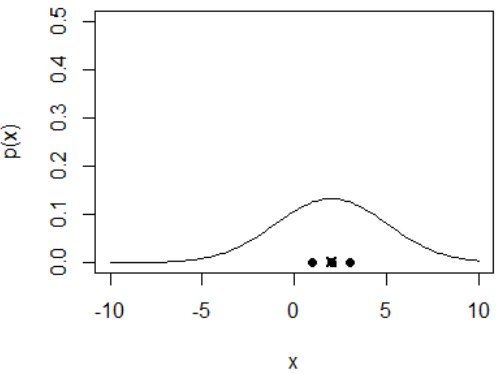
\includegraphics{screenshot007}
			\end{center}
			\item $\mu_\text{MLE} = \dfrac{\sum_{i=1}^{n}x_i}{n} = \dfrac{1+2+3}{3} = 2$.
			
			$\sigma_\text{MLE}^2 = \dfrac{\sum_{i=1}^{n}(x_i - \mu_\text{MLE})^2}{n} = \dfrac{(1-2)^2 + (2-2)^2 + (3-2)^2}{3} = \dfrac{2}{3}$.
			\begin{center}
				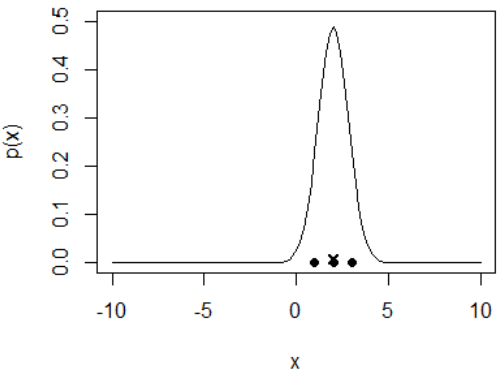
\includegraphics{screenshot008}
			\end{center}
			
			
		\end{enumerate}
		\newpage
		\item \textbf{Rezolvare Exercițiul 3}
		
		\textbf{Metoda 1:}
		
		$\theta_\text{MLE} = \dfrac{\#(X=1)}{\text{număr rânduri}} = \dfrac{1}{4}$
		
		\textbf{Metoda 2:}
		
		Aplicăm următorul \textbf{algoritm EM}:
		
		\begin{algorithmic}
			\STATE Initialization: $\theta^{(0)}\gets 0$
			\FOR{t = 1:maxIterations} 
			\STATE {$\theta^{(t)} \gets \dfrac{\#(X=1) + \#(X=NA) \theta^{(t-1)}}{\#(X=0) + \#(X=1) + \#(X=NA)} \left(== \dfrac{1 + \theta^{(t-1)}}{5}\right)$} 
			\ENDFOR
		\end{algorithmic}
		
		Astfel, obținem $\theta^{(0)} = 0 \rightarrow \theta^{(1)} = 0.2 \rightarrow \theta^{(2)} = 0.24 \rightarrow \dots \rightarrow \theta^{(10)} = 0.25 \rightarrow \theta^{(11)} = 0.25$. Cum $\theta^{(10)} == \theta^{(11)}$, algoritmul a convers la 0.25, ceea ce înseamnă că $\theta_\text{MLE} = 0.25$, adică a ieșit cât a zis Metoda 1.
		
		\item \textbf{Rezolvare Exercițiul 4}
		
		Pe cazul general, notăm cu $n$ numărul de rânduri.
		\begin{enumerate}
			\item $\mu_\text{1;MLE} = \dfrac{\sum_{i=1}^n{1\{y_i=1\} x_i}}{{\sum_{i=1}^n}{1\{y_i=1\}}} = \dfrac{1+3}{2} = 2$
			
			$\mu_\text{2;MLE} = \dfrac{\sum_{i=1}^n{1\{y_i=2\} x_i}}{{\sum_{i=1}^n}{1\{y_i=2\}}} = \dfrac{10+12}{2} = 11$
			
			\newpage
			
			Graficul pentru $0.25 \cdot \mathcal{N}(x;2,1^2)$ și $0.75 \cdot \mathcal{N}(x;11,4^2)$:
								
			\begin{center}
				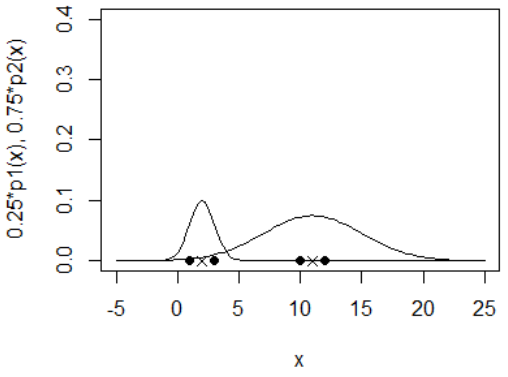
\includegraphics{screenshot009}
			\end{center}
			
			
			\item 
			
			$\pi_\text{1;MLE} = \dfrac{\sum_{i=1}^{n}1\{y_i=1\}}{n} = \dfrac{2}{4} = \dfrac{1}{2}$
			
			$\pi_\text{2;MLE} = \dfrac{\sum_{i=1}^{n}1\{y_i=2\}}{n} = \dfrac{2}{4} = \dfrac{1}{2}$
			
			$\mu_\text{1;MLE} = \dfrac{\sum_{i=1}^n{1\{y_i=1\} x_i}}{{\sum_{i=1}^n}{1\{y_i=1\}}} = \dfrac{1+3}{2} = 2$
			
			$\mu_\text{2;MLE} = \dfrac{\sum_{i=1}^n{1\{y_i=2\} x_i}}{{\sum_{i=1}^n}{1\{y_i=2\}}} = \dfrac{10+12}{2} = 11$
			
			$\sigma^2_\text{1;MLE} = \dfrac{\sum_{i=1}^{n} 1\{y_i=1\} (x_i - \mu_\text{1;MLE})}{{\sum_{i=1}^n}{1\{y_i=1\}}} =\dfrac{(1-2)^2 + (3-2)^2}{2} = 1$
			$$\sigma^2_\text{2;MLE} = \dfrac{\sum_{i=1}^{n} 1\{y_i=2\} (x_i - \mu_\text{2;MLE})}{{\sum_{i=1}^n}{1\{y_i=2\}}} =\dfrac{(10-11)^2 + (12-11)^2}{2} = 1$$
			
			\newpage
			
			Graficul pentru $0.5 \cdot \mathcal{N}(x;2,1^2)$ și $0.5 \cdot \mathcal{N}(x;11,1^2)$:
			
			\begin{center}
				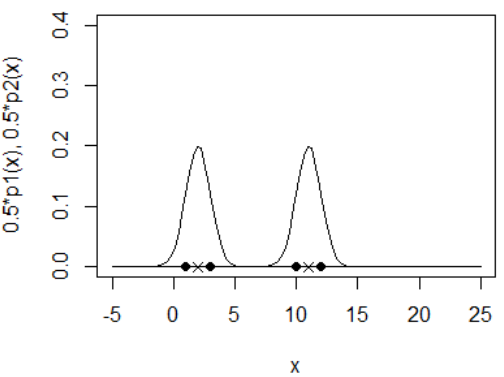
\includegraphics{screenshot010}
			\end{center}
			
			
			\textbf{Observație}: Puteți introduce datele în următoarea aplicație web pentru a obține rezultatele finale și un grafic ajutător: \url{https://ml-fii.shinyapps.io/gnb_1d/}.
			
		\end{enumerate}
		
		\item \textbf{Rezolvare Exercițiul 5}
		
		Pe cazul general, notăm cu $n$ numărul de rânduri.
		
		\begin{enumerate}
			\item \textbf{Metoda 1:} --
			
			\textbf{Metoda 2:}
			
			Aplicăm următorul \textbf{algoritm EM/GMM (doar $\mu$-urile variază)}:
			\begin{algorithmic}
				\STATE Initialization: $\mu_1^{(0)}\gets 0$, $\mu_2^{(0)}\gets 9$
				\FOR{t = 1:maxIterations} 
				\STATE \textbf{E step}: Compute $\gamma_{ij} \stackrel{\text{not.}}{=} E_{Z_i|X_i=x_i,\mu_1^{(t-1)},\mu_2^{(t-1)} }[1\{Z_i=j\}]$, $\forall i \in \{1,2,3,4\}, j\in \{1,2\}$
				\STATE \textbf{M step}: $\mu_1^{(t)} \gets \dfrac{\sum_{i=1}^{n} \gamma_{i1} x_i}{\sum_{i=1}^{n} \gamma_{i1}}$, $\mu_2^{(t)} \gets \dfrac{\sum_{i=1}^{n} \gamma_{i2} x_i}{\sum_{i=1}^{n} \gamma_{i2}}$
				\ENDFOR
			\end{algorithmic}
		
			Considerăm știute următoarele aproximări:
			
			\begin{tabular}{ |c|c|c|c|c|c|c|c|c| } 
				\hline
				x & 0.25 & 0.75 & 1 & 1.5 & 2 & 3 & 10 & 12 \\ 
				\hline
				$\mathcal{N}(x;0,1)$ & 0.386 & 0.301 & 0.241 & 0.129 & 0.053 & 0.004 & 0 & 0 \\ 
				\hline
			\end{tabular}
		
			\textbf{Inițializare}: $\mu_1^{(0)} = 0$, $\mu_2^{(0)} = 9$
		
			\textbf{Pas E}:
			
			Mai întâi, calculăm $\mathcal{N}(x_i;0,1)$, $\mathcal{N}(x_i;9,4^2)$, $i \in\{1,2,3,4\}$:
			
			$\begin{cases}
				\mathcal{N}(1;0,1) \approx 0.241\\
				\mathcal{N}(1;9,4^2) = \dfrac{1}{4} \mathcal{N}\left(\dfrac{1-9}{4};0,1\right) = \dfrac{1}{4} \mathcal{N}\left(-2;0,1\right) = \dfrac{1}{4} \mathcal{N}\left(2;0,1\right) \approx \dfrac{0.053}{4} \approx 0.013
			\end{cases}$

			$\begin{cases}
			\mathcal{N}(3;0,1) \approx 0.004\\
			\mathcal{N}(3;9,4^2) = \dfrac{1}{4} \mathcal{N}\left(\dfrac{3-9}{4};0,1\right) = \dfrac{1}{4} \mathcal{N}\left(-1.5;0,1\right) = \dfrac{1}{4} \mathcal{N}\left(1.5;0,1\right) \approx \dfrac{0.129}{4} \approx 0.032
			\end{cases}$
		
			$\begin{cases}
			\mathcal{N}(10;0,1) \approx 0\\
			\mathcal{N}(10;9,4^2) = \dfrac{1}{4} \mathcal{N}\left(\dfrac{10-9}{4};0,1\right) = \dfrac{1}{4} \mathcal{N}\left(0.25;0,1\right) \approx \dfrac{0.386}{4} \approx 0.096
			\end{cases}$
		
			$\begin{cases}
			\mathcal{N}(12;0,1) \approx 0\\
			\mathcal{N}(12;9,4^2) = \dfrac{1}{4} \mathcal{N}\left(\dfrac{12-9}{4};0,1\right) = \dfrac{1}{4} \mathcal{N}\left(0.75;0,1\right) \approx \dfrac{0.301}{4} \approx 0.075
			\end{cases}$
		
			Apoi calculăm $\gamma_{ij}$, $i\in\{1,2,3,4\}, j \in \{1,2\}$:
			
			$$\gamma_{ij} = \frac{\pi_j  \mathcal{N}(x_i;\mu^{(0)}_j,\sigma_j^2)}{ 1/4 \cdot \mathcal{N}(x_i;0,1) + 3/4 \cdot \mathcal{N}(x_i;9,4^2) }$$
			
			\begin{tabular}{ |c|c|c| } 
				\hline
				$\gamma_{ij}$ & $\mathcal{N}_1$ & $\mathcal{N}_2$ \\ 
				\hline
				$x_1 = 1$ & $\dfrac{1/4 \cdot 0.241}{1/4 \cdot 0.241 + 3/4 \cdot 0.013} \approx 0.86$ & $\dfrac{3/4 \cdot 0.013}{1/4 \cdot 0.241 + 3/4 \cdot 0.013} \approx 0.14$ \\
				$x_2 = 3$ & $\dfrac{1/4 \cdot 0.004}{1/4 \cdot 0.004 + 3/4 \cdot 0.032} \approx 0.04$ & $\dfrac{3/4 \cdot 0.032}{1/4 \cdot 0.004 + 3/4 \cdot 0.032} \approx 0.96$ \\
				$x_3 = 10$ & $\dfrac{1/4 \cdot 0}{1/4 \cdot 0 + 3/4 \cdot 0.096} \approx 0$ & $\dfrac{3/4 \cdot 0.096}{1/4 \cdot 0 + 3/4 \cdot 0.096} \approx 1$ \\
				$x_4 = 12$ &$\dfrac{1/4 \cdot 0}{1/4 \cdot 0 + 3/4 \cdot 0.075} \approx 0$ & $\dfrac{3/4 \cdot 0.075}{1/4 \cdot 0 + 3/4 \cdot 0.075} \approx 1$ \\
				\hline
			\end{tabular}

			\textbf{Pas M}:
			$$\mu_1^{(1)} = \frac{0.86 \cdot 1 + 0.04 \cdot 3 + 0 \cdot 10 + 0 \cdot 12}{0.86 + 0.04 + 0 + 0} \approx 1.088$$
			$$\mu_2^{(1)} = \frac{0.14 \cdot 1 + 0.96 \cdot 3 +1 \cdot 10 + 1 \cdot 12}{0.14 + 0.96 + 1 + 1} \approx 8.070$$
			
			Se execută iterații până la convergență.
			
			Graficul (de la iterația 0 - inițializare) pentru $0.25 \cdot \mathcal{N}(x;0,1^2)$ și $0.75 \cdot \mathcal{N}(x;9,4^2)$:
			
		\begin{center}
			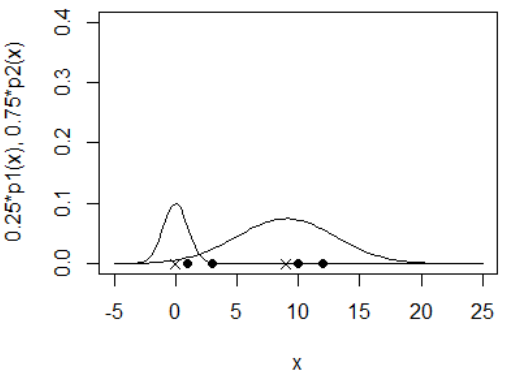
\includegraphics{screenshot012}
		\end{center}
		
			
			\newpage
			Graficul (de la iterația 1) pentru $0.25 \cdot \mathcal{N}(x;1.088,1^2)$ și $0.75 \cdot \mathcal{N}(x;8.070,4^2)$:
			\begin{center}
				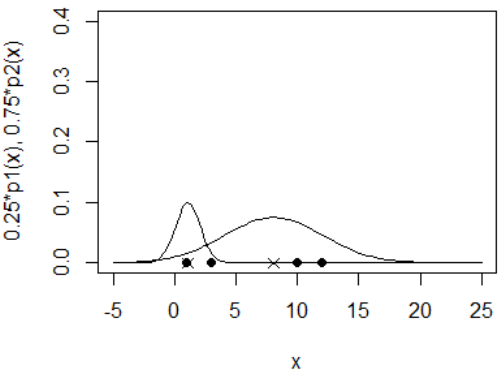
\includegraphics[width=0.8\linewidth]{screenshot013}
			\end{center}
			
			
			
			\textbf{Observație}: Puteți introduce datele în următoarea aplicație web pentru a obține rezultatele de la pașii E și M și grafice ajutătoare: \url{https://ml-fii.shinyapps.io/emApp/}. Trebuie să selectați \textit{Fix pis} și \textit{Fix sigmas} pentru a lăsă doar $\mu$-urile să varieze.
			
			\item Aplicăm următorul \textbf{algoritm EM (toți parametrii variază)}:
			\begin{algorithmic}
				\STATE Initialization: 
				
				$\pi_1^{(0)}\gets 1/4$, $\pi_2^{(0)}\gets 3/4$
				
				$\mu_1^{(0)}\gets 0$, $\mu_2^{(0)}\gets 9$
				
				$(\sigma_1^2)^{(0)}\gets 1^2$, $(\sigma_2^2)^{(0)}\gets 4^2$
				
				\FOR{t = 1:maxIterations} 
				\STATE \textbf{E step}: Compute $\gamma_{ij}$, $\forall i \in \{1,2,3,4\}, j\in \{1,2\}$
				\STATE \textbf{M step}: 
				
				$\pi_1^{(t)} \gets \dfrac{\sum_{i=1}^{n} \gamma_{i1}}{n}$, $\pi_2^{(t)} \gets \dfrac{\sum_{i=1}^{n} \gamma_{i2}}{n}$
				
				$\mu_1^{(t)} \gets \dfrac{\sum_{i=1}^{n} \gamma_{i1} x_i}{\sum_{i=1}^{n} \gamma_{i1}}$, $\mu_2^{(t)} \gets \dfrac{\sum_{i=1}^{n} \gamma_{i2} x_i}{\sum_{i=1}^{n} \gamma_{i2}}$
				
				$(\sigma_1^2)^{(t)} \gets \dfrac{\sum_{i=1}^{n} \gamma_{i1} (x_i - \mu_1^{(t)})^2}{\sum_{i=1}^{n} \gamma_{i1}}$, $(\sigma_2^2)^{(t)} \gets \dfrac{\sum_{i=1}^{n} \gamma_{i2} (x_i - \mu_2^{(t)})^2}{\sum_{i=1}^{n} \gamma_{i2}}$
				\ENDFOR
			\end{algorithmic}
		
			\textbf{Inițializare}:
		
			$\pi_1^{(0)}\gets 1/4$, $\pi_2^{(0)}\gets 3/4$
			
			$\mu_1^{(0)}\gets 0$, $\mu_2^{(0)}\gets 9$
			
			$(\sigma_1^2)^{(0)}\gets 1^2$, $(\sigma_2^2)^{(0)}\gets 4^2$
			
			\textbf{Pas E}: exact ca la subpunctul precedent
			
			\textbf{Pas M}: 
			$$\pi_1^{(1)} = \dfrac{0.86 + 0.04 + 0+ 0}{4} = 0.225$$
			$$\pi_2^{(1)} = \dfrac{0.14 + 0.96 + 1+ 1}{4} = 0.775$$
			$$\mu_1^{(1)} = \frac{0.86 \cdot 1 + 0.04 \cdot 3 + 0 \cdot 10 + 0 \cdot 12}{0.86 + 0.04 + 0 + 0} \approx 1.088$$
			$$\mu_2^{(1)} = \frac{0.14 \cdot 1 + 0.96 \cdot 3 +1 \cdot 10 + 1 \cdot 12}{0.14 + 0.96 + 1 + 1} \approx 8.070$$
			$$(\sigma^2_1)^{(1)} = \frac{0.86 \cdot (1 - 1.088)^2 + 0.04 \cdot (3-1.088)^2 + 0 \cdot (10 - 1.088)^2 + 0 \cdot (12 - 1.088)^2}{0.86 + 0.04 + 0 + 0}$$
			$$\approx 0.169$$
			$$(\sigma^2_2)^{(1)} = \frac{0.14 \cdot (1 - 8.070)^2 + 0.96 \cdot (3-8.070)^2 + 1 \cdot (10 - 8.070)^2 + 1 \cdot (12 - 8.070)^2}{0.14 + 0.96 + 1 + 1}$$
			$$\approx 16.401$$
			
			Se execută iterații până la convergență.
			
	\textbf{Observație}: Puteți introduce datele în următoarea aplicație web pentru a obține rezultatele de la pașii E și M și grafice ajutătoare: \url{https://ml-fii.shinyapps.io/emApp/}.
\newpage

			Graficul (de la iterația 0 - inițializare) pentru $0.25 \cdot \mathcal{N}(x;0,1^2)$ și $0.75 \cdot \mathcal{N}(x;9,4^2)$:
			\begin{center}
				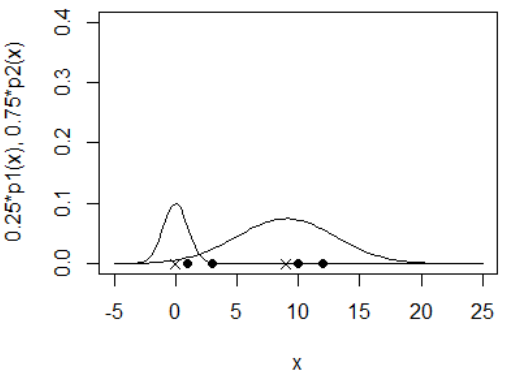
\includegraphics{screenshot012}
			\end{center}
			Graficul (de la iterația 1) pentru $0.225 \cdot \mathcal{N}(x;1.088,0.169)$ și $0.775 \cdot \mathcal{N}(x;8.070,16.401)$:
			\begin{center}
				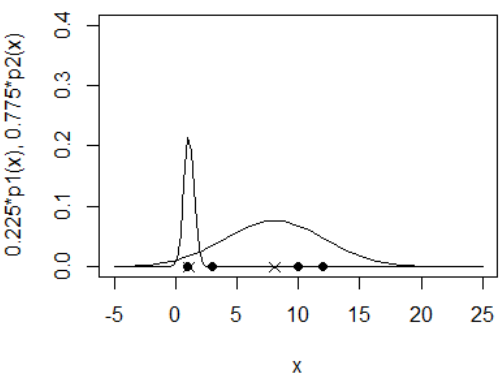
\includegraphics{screenshot014}
			\end{center}
			
			
		
			
		\end{enumerate}

			
		
	\end{enumerate}

\newpage

	\subsubsection{Derivare formule/algoritmi}
	\begin{enumerate}
		\item \textbf{Derivare formule/algoritmi Exercițiu 1}
		
		parametrii: $\theta$
		
		$\theta_\text{MLE} = \arg \max_{\theta \in [0,1]} \underbrace{L_D(\theta)}_\text{f. de verosimilitate/likelihood} = \arg \max_{\theta \in [0,1]} \underbrace{l_D(\theta)}_\text{f. de log-verosimiltate/log-likelihood}$
		
		\begin{align*}
		L_D(\theta) &\stackrel{\text{def.}}{=} p(D|\theta)\\
		&=p_{X_1,X_2,X_3,X_4}(x_1,x_2,x_3,x_4|\theta)\\
		&\stackrel{\text{indep.}}{=}p_{X_1}(x_1|\theta) p_{X_2}(x_2|\theta) p_{X_3}(x_3|\theta) p_{X_4}(x_4|\theta)\\
		&=p_{X_1}(0|\theta) p_{X_2}(0|\theta) p_{X_3}(0|\theta) p_{X_4}(1|\theta)\\
		&=(1-\theta)(1-\theta)(1-\theta)\theta\\
		&=(1-\theta)^3 \theta\\
		l_D(\theta) &\stackrel{\text{def.}}{=} \ln L_D(\theta)\\
		&=\ln \left((1-\theta)^3 \theta\right)\\
		&=3 \ln(1-\theta) + \ln \theta
		\end{align*}
		
		Pentru a maximiza $l_D$ vom folosi derivate:
		
		$l_D'(\theta) = \dfrac{3}{1-\theta}(-1) + \dfrac{1}{\theta} = \dfrac{1}{\theta} - \dfrac{3}{1-\theta}$.
		
		$l_D'(\theta) = 0 \Rightarrow \dfrac{1}{\theta} = \dfrac{3}{1-\theta} \Rightarrow \dfrac{1-\theta}{\theta} = \dfrac{3}{1} \stackrel{\text{adună numitor la numărător}}{\Rightarrow} \dfrac{1}{\theta} = \dfrac{4}{1} \Rightarrow \hat{\theta} = \dfrac{1}{4} \in [0,1]$.
		
		Verificăm dacă $\hat{\theta}$ este punct de maxim.
		
		$l_D''(\theta) = (\theta^{-1} - 3(1-\theta)^{-1})' = (-1)\theta^{-2} - 3(-1)(1-\theta)^{-2}(-1) = -\dfrac{1}{\theta^2} - \dfrac{3}{(1-\theta)^2} < 0, \forall \theta \in [0,1] \Rightarrow l_D\text{-concavă} \Rightarrow \hat{\theta} = \dfrac{1}{4}$ este punct de maxim.
		
		Deci, $\theta_\text{MLE} = \dfrac{1}{4}$.
		
		\newpage
		
		\item \textbf{Derivare formule/algoritmi Exercițiu 2}
		
		parametrii: $\mu$

		$\mu_\text{MLE} = \arg \max_{\mu \in \mathbb{R}} L_D(\mu) = \arg \max_{\mu \in \mathbb{R}} l_D(\mu)$
		
		\begin{align*}
		L_D(\mu) &\stackrel{\text{def.}}{=} p(D|\mu)\\
		&=p_{X_1,X_2,X_3}(x_1,x_2,x_3|\mu)\\
		&\stackrel{\text{indep.}}{=}p_{X_1}(x_1|\mu) p_{X_2}(x_2|\mu) p_{X_3}(x_3|\mu)\\
		&=p_{X_1}(1|\mu) p_{X_2}(2|\mu) p_{X_3}(3|\mu)\\
		&=\dfrac{1}{\sqrt{2\pi} 3} e^{-\frac{1}{2}\left(\frac{1-\mu}{3}\right)^2}  \dfrac{1}{\sqrt{2\pi} 3} e^{-\frac{1}{2}\left(\frac{2-\mu}{3}\right)^2} \dfrac{1}{\sqrt{2\pi} 3} e^{-\frac{1}{2}\left(\frac{3-\mu}{3}\right)^2}\\
		&=\left(\frac{1}{\sqrt{2\pi}3}\right)^3 e^{-\frac{1}{2\cdot 3^2} ((1-\mu)^2 + (2-\mu)^2 + (3-\mu)^2) }\\
		&=\left(\frac{1}{\sqrt{2\pi}3}\right)^3 e^{-\frac{1}{2\cdot 3^2} (3\mu^2 - 12\mu + 14) }\\
		l_D(\mu) &\stackrel{\text{def.}}{=} \ln L_D(\mu)\\
		&=\ln\left( \left(\frac{1}{\sqrt{2\pi}3}\right)^3 e^{-\frac{1}{2\cdot 3^2} (3\mu^2 - 12\mu + 14) }\right)\\
		&=-3\ln(\sqrt{2 \pi} 3) - \frac{1}{2\cdot 3^3} (3\mu^2 - 12 \mu + 14)
		\end{align*}
		
		Pentru a maximiza $l_D$ putem folosi derivate SAU putem proceda astfel:
		\begin{align*}
		\arg \max_{\mu \in \mathbb{R}} l_D(\mu) &= \arg \max_{\mu \in \mathbb{R}} -\frac{1}{2 \cdot 3^2}(3\mu^2 - 12 \mu + 14) \\
		&= \arg \min_{\mu \in \mathbb{R}}(3\mu^2 - 12 \mu + 14)\\
		&=-\frac{b}{2a} = -\frac{-12}{2\cdot 3}=2
		\end{align*}
		
		Deci, $\mu_\text{MLE} = 2$.
		
		\newpage
		
		\item \textbf{Derivare formule/algoritmi Exercițiu 3}
		
		\textbf{Metoda 1}:
		
		$\theta_\text{MLE} = \arg \max_{\theta \in [0,1]} L_D(\theta) = \arg \max_{\theta \in [0,1]} l_D(\theta)$
		\begin{align*}
		L_D(\theta) &\stackrel{\text{def.}}{=} p(D|\theta)\\
		&=p_{X_1,X_2,X_3,X_4}(x_1,x_2,x_3,x_4|\theta)\\
		&\stackrel{\text{indep.}}{=}p_{X_1}(x_1|\theta) p_{X_2}(x_2|\theta) p_{X_3}(x_3|\theta) p_{X_4}(x_4|\theta)\\
		&=p_{X_1}(0|\theta) p_{X_2}(0|\theta) p_{X_3}(0|\theta) p_{X_4}(1|\theta)\\
		&=(1-\theta)(1-\theta)(1-\theta)\theta\\
		&=(1-\theta)^3 \theta
		\end{align*}
		Observăm că am obținut aceeași funcție de verosimilitate ca la Exercițiul 1.
		
		Din Exercițiul 1 avem că $\theta_\text{MLE} = \dfrac{1}{4}$.
		\\--------------------------------------------------------------------------------------------\\
		\textbf{Metoda 2}:
		
		parametrii: $\theta$
		
		$\theta_\text{MLE} = \arg \max_{\theta \in[0,1]} L_D(\theta)$
		
		Pentru a maximiza $L_D$ vom folosi algoritmul EM care este un algoritm iterativ:
		
		0. Vom porni cu inițializarea $\theta^{(0)} = 0$
		
		La iterația $t$:
		
		\textbf{Pas E}:
		
		1. Calculăm funcțiile de verosimiliate și log-verosimilitate a datelor \textbf{complete}.
		
		\begin{align*}
		L_{D_c}(\theta) &\stackrel{\text{def.}}{=} p(D_c|\theta)\\
		&=p_{X_1,X_2,X_3,X_4,Z_1}(x_1,x_2,x_3,x_4,Z_1|\theta)\\
		&\stackrel{\text{indep.}}{=}p_{X_1}(x_1|\theta) p_{X_2}(x_2|\theta) p_{X_3}(x_3|\theta) p_{X_4}(x_4|\theta) p_{Z_1}(Z_1|\theta)\\
		&=p_{X_1}(0|\theta) p_{X_2}(0|\theta) p_{X_3}(0|\theta) p_{X_4}(1|\theta) p_{Z_1}(Z_1|\theta)\\
		&=(1-\theta)(1-\theta)(1-\theta)\theta (1-\theta)^{1-Z_1}\theta^{Z_1}\\
		&=(1-\theta)^{4-Z_1} \theta^{1+Z_1}\\
		l_{D_c}(\theta) &\stackrel{\text{def.}}{=} \ln L_{D_c}(\theta)\\
		&=\ln \left((1-\theta)^{4-Z_1} \theta^{1+Z_1}\right)\\
		&=(4-Z_1) \ln(1-\theta) + (1+Z_1)\ln \theta
		\end{align*}
		2. După cum se poate observa $l_{D_c}$ este o VA (pentru că $Z_1$ este VA). Pentru a scăpa de acest \textit{neajuns} aplicăm ``E" (\textit{expectation}/media unei VA) peste $l_{D_c}$ și astfel obținem o funcție cu valori în $\mathbb{R}$ pe care o putem maximiza. ``E" va fi aplicat cu privire la distribuția ``latent$|$observabil,parametri\_it\_trecută", adică ``$Z_1|X_1=x_1,X_2=x_2,X_3=x_3,X_4=x_4,\theta^{(t-1)}$" în cazul nostru. Cum $Z_1,X_1,X_2,X_3,X_4$ sunt independente avem că ``$Z_1|X_1=x_1,X_2=x_2,X_3=x_3,X_4=x_4,\theta^{(t-1)}$" este ``$Z_1|\theta^{(t-1)}$".
		\begin{align*}
		E_{Z_1|X_1=x_1,X_2=x_2,X_3=x_3,X_4=x_4,\theta^{(t-1)}}&[l_{D_c}(\theta)] = E_{Z_1|\theta^{(t-1)}}[l_{D_c}(\theta)]\\
		&=E_{Z_1|\theta^{(t-1)}}[(4-Z_1) \ln(1-\theta) + (1+Z_1)\ln \theta]\\
		&\stackrel{\text{lin.E}}{=}(4-E_{Z_1|\theta^{(t-1)}}[Z_1]) \ln(1-\theta) + (1+E_{Z_1|\theta^{(t-1)}}[Z_1])\ln \theta\\
		E_{Z_1|\theta^{(t-1)}}[Z_1] &= 0 \cdot P(Z_1 = 0|\theta^{(t-1)}) + 1\cdot P(Z_1 = 1|\theta^{(t-1)})\\
		& = P(Z_1 = 1|\theta^{(t-1)})\\
		& = \theta^{(t-1)}\\
		E_{Z_1|X_1=x_1,X_2=x_2,X_3=x_3,X_4=x_4,\theta^{(t-1)}}&[l_{D_c}(\theta)] = (4 - \theta^{(t-1)}) \ln(1-\theta) + (1+\theta^{(t-1)}) \ln \theta\\
		&\stackrel{\text{not.}}{=} Q(\theta|\theta^{(t-1)}) \stackrel{\text{sau simplu}}{=} Q(\theta)
		\end{align*}
		
		\textbf{Pas M}:
		
		3. Maximizăm funcția $Q(\theta|\theta^{(t-1)})$. Vom folosi derivate:
		
		$Q'(\theta) = \dfrac{4 - \theta^{(t-1)}}{1-\theta} (-1) + \dfrac{1 + \theta^{(t-1)}}{\theta} = \dfrac{1 + \theta^{(t-1)}}{\theta} - \dfrac{4 - \theta^{(t-1)}}{1-\theta}$
		
		$Q'(\theta) = 0 \Rightarrow \dfrac{1 + \theta^{(t-1)}}{\theta} = \dfrac{4 - \theta^{(t-1)}}{1-\theta} \Rightarrow \dfrac{1-\theta}{\theta} = \dfrac{4 - \theta^{(t-1)}}{1 + \theta^{(t-1)}} \stackrel{\text{adună numitor la numărător}}{\Rightarrow} \dfrac{1}{\theta} = \dfrac{5}{1+\theta^{(t-1)}} \Rightarrow \hat{\theta} = \dfrac{1 + \theta^{(t-1)}}{5} \in [0,1]$
		
		Verificăm dacă $\hat{\theta}$ este punct de maxim.
		\begin{align*}
		Q''(\theta) &= ((1 + \theta^{(t-1)})\theta^{-1} - (4 - \theta^{(t-1)})(1-\theta)^{-1})'\\
		&=(1+\theta^{(t-1)})(-1)\theta^{-2} - (4-\theta^{(t-1)})(-1)(1-\theta)^{-2}(-1)\\
		&=-\dfrac{1+\theta^{(t-1)}}{\theta^2} - \dfrac{4-\theta^{(t-1)}}{(1-\theta)^2} <0,\forall \theta \in[0,1] \Rightarrow Q\text{ - concavă} \Rightarrow \hat{\theta}\text{ este punct de maxim.}
		\end{align*}
		
		Deci, $\theta^{(t)} = \dfrac{1+\theta^{(t-1)}}{5}$.
		
		Am obținut astfel următorul \textbf{algoritm EM}:
		
		\begin{algorithmic}
			\STATE Initialization: $\theta^{(0)}\gets 0$
			\FOR{t = 1:maxIterations} 
			\STATE {$\theta^{(t)} \gets  \dfrac{1 + \theta^{(t-1)}}{5}$} 
			\ENDFOR
		\end{algorithmic}
		
		\textbf{Observație}: Acesta este unul dintre cele mai simple exemple de derivare a algoritmului EM. Deși aici acest lucru a fost nefolositor pentru că există deja Metoda 1, în alte cazuri (spre exemplu, în cadrul mixturii de gaussiene) Metoda 1 nu ne dă o formulă analitică (\textit{closed-form}) pentru parametri, așa că o alternativă este algoritmul EM.
			
		
		\newpage
		
		\item \textbf{Derivare formule/algoritmi Exercițiu 4}
		
		(a)
		
		parametrii: $\mu_1, \mu_2$
		
		$(\mu_\text{1;MLE},\mu_\text{2;MLE}) = \arg \max_{(\mu_1,\mu_2) \in \mathbb{R}^2} L_D(\mu_1,\mu_2) = \arg \max_{(\mu_1,\mu_2) \in \mathbb{R}^2} l_D(\mu_1,\mu_2)$
		\begin{align*}
		L_D(\mu_1,\mu_2) &\stackrel{\text{def.}}{=} p_{(X_1,Y_1),(X_2,Y_2),(X_3,Y_3),(X_4,Y_4)}((x_1,y_1),(x_2,y_2),(x_3,y_3),(x_4,y_4)|\mu_1,\mu_2)\\
		&\stackrel{\text{indep.}}{=} p_{X_1,Y_1}(x_1,y_1) p_{X_2,Y_2}(x_2,y_2) p_{X_3,Y_3}(x_3,y_3) p_{X_4,Y_4}(x_4,y_4)\\
		&=p_{X_1,Y_1}(1,1) p_{X_2,Y_2}(3,1) p_{X_3,Y_3}(10,2) p_{X_4,Y_4}(12,2)\\
		&\stackrel{\text{f.de înmulț.}}{=} p_{Y_1}(1) p_{X_1|Y_1}(1|1)  p_{Y_2}(1) p_{X_2|Y_2}(3|1)  p_{Y_3}(2) p_{X_3|Y_3}(10|2)  p_{Y_4}(2) p_{X_4|Y_4}(12|2)\\
		&=\dfrac{1}{4} \dfrac{1}{\sqrt{2\pi}1} e^{-\frac{1}{2}\left(\frac{1-\mu_1}{1}\right)^2}
		\dfrac{1}{4} \dfrac{1}{\sqrt{2\pi}1} e^{-\frac{1}{2}\left(\frac{3-\mu_1}{1}\right)^2}
		\dfrac{3}{4} \dfrac{1}{\sqrt{2\pi}4} e^{-\frac{1}{2}\left(\frac{10-\mu_2}{4}\right)^2}
		\dfrac{3}{4} \dfrac{1}{\sqrt{2\pi}4} e^{-\frac{1}{2}\left(\frac{12-\mu_2}{4}\right)^2}\\
		&=\left(\dfrac{1}{4}\right)^2 \left(\dfrac{3}{4}\right)^2 \left(\dfrac{1}{\sqrt{2\pi 1}}\right)^2 \left(\dfrac{1}{\sqrt{2\pi 4}}\right)^2 e^{-\frac{1}{2}\left((1-\mu_1)^2 + (3-\mu_1)^2 + \frac{1}{4^2} \left(\left({10-\mu_2}\right)^2 + \left({12-\mu_2}\right)^2\right) \right)}\\
		&=\text{const.}\cdot e^{-\frac{1}{2}\left(2\mu_1^2 - 8\mu_1 + 10 + \frac{1}{4^2} \left(2\mu_2^2 - 44\mu_2 + 244\right) \right)}\\
		l_D(\mu_1,\mu_2) &\stackrel{\text{def.}}{=} \ln L_D(\mu_1,\mu_2)\\
		& =\ln(\text{const.}) - \frac{1}{2}\left(2\mu_1^2 - 8\mu_1 + 10 + \frac{1}{4^2} \left(2\mu_2^2 - 44\mu_2 + 244\right) \right)
		\end{align*}
		Pentru a maximiza $l_D$ putem folosi derivate SAU putem proceda astfel:
		$\arg \max_{(\mu_1,\mu_2)\in \mathbb{R}^2} l_D(\mu_1,\mu_2) =$
		\begin{align*}
		&= \arg \max_{(\mu_1,\mu_2)\in \mathbb{R}^2}  - \frac{1}{2}\left(2\mu_1^2 - 8\mu_1 + 10 + \frac{1}{4^2} \left(2\mu_2^2 - 44\mu_2 + 244\right) \right)\\
		&=\arg \min_{(\mu_1,\mu_2)\in \mathbb{R}^2} \left(2\mu_1^2 - 8\mu_1 + 10 + \frac{1}{4^2} \left(2\mu_2^2 - 44\mu_2 + 244\right) \right)\\
		&\stackrel{\text{$\mu_1$ nu \textit{interacț.} cu $\mu_2$}}{=} \begin{bmatrix}
		\arg \min_{\mu_1 \in \mathbb{R}} (2\mu_1^2 - 8\mu_1 + 10)\\
		\arg \min_{\mu_2 \in \mathbb{R}} (2\mu_2^2 - 44\mu_2 + 244)\\
		\end{bmatrix}\\
		&=\begin{bmatrix}
		-\dfrac{b_1}{2a_1}\\
		-\dfrac{b_2}{2a_2}
		\end{bmatrix}=\begin{bmatrix}
		-\dfrac{-8}{4}\\
		-\dfrac{-44}{4}
		\end{bmatrix}=\begin{bmatrix}
		2\\
		11
		\end{bmatrix}
		\end{align*}
		
		Deci, $\mu_\text{1;MLE} = 2$, $\mu_\text{2;MLE} = 11$.
		

		
		\item \textbf{Derivare formule/algoritmi Exercițiu 5}
		
		(a)
		
		\textbf{Metoda 1}:
		
		parametrii: $\mu_1,\mu_2$
		
		$(\mu_\text{1;MLE},\mu_\text{2;MLE}) = \arg \max_{(\mu_1,\mu_2) \in \mathbb{R}^2} L_D(\mu_1,\mu_2) = \arg \max l_D(\mu_1,\mu_2)$
		\begin{align*}
		L_D(\mu_1,\mu_2) &\stackrel{\text{def.}}{=} p_{X_1,X_2,X_3,X_4}(x_1,x_2,x_3,x_4|\mu_1,\mu_2)\\
		&\stackrel{\text{indep.}}{=} p_{X_1}(x_1) p_{X_2}(x_2) p_{X_3}(x_3) p_{X_4}(x_4)\\
		&=p_{X_1}(1) p_{X_2}(3) p_{X_3}(10) p_{X_4}(12)\\
		&\stackrel{\text{p.marg.}}{=} (p_{X_1,Z_1}(1,1)+p_{X_1,Z_1}(1,2)) \cdot (p_{X_2,Z_2}(3,1)+p_{X_2,Z_2}(3,2)) \cdot\\
		& \cdot (p_{X_3,Z_3}(10,1)+p_{X_3,Z_3}(10,2)) \cdot (p_{X_4,Z_4}(12,1)+p_{X_4,Z_4}(12,2))\\
		&\stackrel{\text{f.de înmulț.}}{=} \left(p_{Z_1}(1)p_{X_1|Z_1}(1|1) + p_{Z_1}(2) p_{X_1|Z_1}(1|2)\right) \dots
		\end{align*}
		Am putea înlocui mai departe, însă putem observa că ln-ul de la funcția de log-verosimilitate ne va elimina produsele, însă un factor va conține o sumă de termeni cu ``e", ceea ce înseamnă că nu scăpăm de ``e" în funcție de $l_D$. Astfel, derivatele nu vor ieși ``frumos" și, mai grav, nu vom găsi formule analitice pentru $\mu_1$, $\mu_2$. Din această cauză ne trebuie o alternativă: algoritmul EM.
		
		\textbf{Observație 1}: Nu vă recomand să începeți rezolvarea acestui exercițiu cu Metoda 1 în condiții de examen/test. Treceți direct la Metoda 2.
		
		\textbf{Observație 2}: O altă alternativă ar fi ca, după ce calculați derivatele lui $l_D$, să aplicați algoritmul \textit{gradient ascent} (pe care unii dintre voi îl știți de la cursul de rețele neuronale). Totuși, când există date latente și vrei să maximizezi verosimilitatea datelor observabile, atunci e de preferat să se folosească algoritmul EM.
		\\--------------------------------------------------------------------------------------------\\
		\textbf{Metoda 2}:
		
		parametrii: $\mu_1,\mu_2$
		
		$(\mu_\text{1;MLE},\mu_\text{2;MLE}) = \arg \max_{(\mu_1,\mu_2)\in \mathbb{R}^2} L_D(\mu_1,\mu_2)$
		
		Pentru a maximiza $L_D$ vom folosi algoritmul EM care este un algoritm iterativ:
		
		0. Vom porni cu inițializarea $\mu_1^{(0)} = 0$, $\mu_2^{(0)} = 9$.
		
		La iterația $t$:
		
		\textbf{Pas E}:
		
		1. Calculăm funcțiile de verosimiliate și log-verosimilitate a datelor \textbf{complete}.
		
		$L_{D_c}(\mu_1,\mu_2) =$
		\begin{align*}
		&\stackrel{\text{def.}}{=} p(D_c|\mu_1,\mu_2)\\
		&=p_{(X_1,Z_1),(X_2,Z_2),(X_3,Z_3),(X_4,Z_4)}((x_1,Z_1),(x_2,Z_2),(x_3,Z_3),(x_4,Z_4)|\mu_1,\mu_2)\\
		&\stackrel{\text{indep.}}{=}p_{X_1,Z_1}(x_1,Z_1) p_{X_2,Z_2}(x_2,Z_2) p_{X_3,Z_3}(x_3,Z_3) p_{X_4,Z_4}(x_4,Z_4)\\
		&=p_{X_1,Z_1}(1,Z_1) p_{X_2,Z_2}(3,Z_2) p_{X_3,Z_3}(10,Z_3) p_{X_4,Z_4}(12,Z_4)\\
		&\stackrel{\text{f.de înmulț.}}{=}p_{Z_1}(Z_1) p_{X_1|Z_1}(1|Z_1) p_{Z_2}(Z_2) p_{X_2|Z_2}(3|Z_2) p_{Z_3}(Z_3) p_{X_3|Z_3}(10|Z_3) p_{Z_4}(Z_4) p_{X_4|Z_4}(12|Z_4)\\
		&\stackrel{\text{tricks}}{=}
		\underbrace{\left(\dfrac{1}{4}\right)^{1\{Z_1=1\}} \left(\dfrac{3}{4}\right)^{1\{Z_1=2\}}}_{p_{Z_1}(Z_1)} \underbrace{\left(\dfrac{1}{\sqrt{2\pi} 1} e^{-\frac{1}{2} \left(\frac{1-\mu_1}{1}\right)^2}\right)^{1\{Z_1=1\}} \left(\dfrac{1}{\sqrt{2\pi} 4} e^{-\frac{1}{2} \left(\frac{1-\mu_2}{4}\right)^2}\right)^{1\{Z_1=2\}}}_{p_{X_1|Z_1}(1|Z_1)} \cdot\\
		&\cdot \underbrace{\left(\dfrac{1}{4}\right)^{1\{Z_2=1\}} \left(\dfrac{3}{4}\right)^{1\{Z_2=2\}}}_{p_{Z_2}(Z_2)} \underbrace{\left(\dfrac{1}{\sqrt{2\pi} 1} e^{-\frac{1}{2} \left(\frac{3-\mu_1}{1}\right)^2}\right)^{1\{Z_2=1\}} \left(\dfrac{1}{\sqrt{2\pi} 4} e^{-\frac{1}{2} \left(\frac{3-\mu_2}{4}\right)^2}\right)^{1\{Z_2=2\}}}_{p_{X_2|Z_2}(3|Z_2)} \cdot \dots\\
		&l_{D_c}(\mu_1,\mu_2) =\\
		&\stackrel{\text{def.}}{=} \ln L_{D_c} (\mu_1,\mu_2)\\
		&=1\{Z_1 = 1\} \ln\left(\frac{1}{4}\right) + 1\{Z_1 = 2\} \ln\left(\frac{3}{4}\right) + 1\{Z_1 = 1\} \left(-\ln(\sqrt{2\pi }1 - \frac{1}{2} (1 - \mu_1)^2)\right) + \\
		&+1\{Z_1 = 2\} \left(-\ln(\sqrt{2\pi}4 - \frac{1}{2} \left(\frac{1 - \mu_2}{4}\right)^2\right) +\\
		&+1\{Z_2 = 1\} \ln\left(\frac{1}{4}\right) + 1\{Z_2 = 2\} \ln\left(\frac{3}{4}\right) + 1\{Z_2 = 1\} \left(-\ln(\sqrt{2\pi }1 - \frac{1}{2} (3 - \mu_1)^2)\right) + \\
		&+1\{Z_2 = 2\} \left(-\ln(\sqrt{2\pi }4 - \frac{1}{2} \left(\frac{3 - \mu_2}{4}\right)^2\right) + \dots
		\end{align*}
		
		2. După cum se poate observa $l_{D_c}$ este o VA (pentru că $Z_1, Z_2, Z_3, Z_4$ sunt VA). Pentru a scăpa de acest \textit{neajuns} aplicăm ``E" (\textit{expectation}/media unei VA) peste $l_{D_c}$ și astfel obținem o funcție cu valori în $\mathbb{R}^2$ pe care o putem maximiza. ``E" va fi aplicat cu privire la distribuția\\ ``latent$|$observabil,parametri\_it\_trecută", adică 
		
		\noindent``$Z_1,Z_2,Z_3,Z_4|X_1=x_1,X_2=x_2,X_3=x_3,X_4=x_4,\mu_1^{(t-1)},\mu_2^{(t-1)}$" în cazul nostru. Cum $(X_1,Z_1),(X_2,Z_2),(X_3,Z_3),(X_4,Z_4)$ sunt independente avem că ``$E_{Z_1,Z_2,Z_3,Z_4|X_1=x_1,X_2=x_2,X_3=x_3,X_4=x_4,\mu_1^{(t-1)},\mu_2^{(t-1)}}[1\{Z_i = j\}]$" este ``$E_{Z_i|X_i=x_i,\mu_1^{(t-1)},\mu_2^{(t-1)}}[1\{Z_i = j\}] \stackrel{\text{not.}}{=}\gamma_{ij}$".
		
		Mai mult:
		\begin{align*}
		\gamma_{ij} &= E_{Z_i|X_i=x_i,\mu_1^{(t-1)},\mu_2^{(t-1)}}[1\{Z_i=j\}]\\
		&=0 \cdot P(1\{Z_i=j\} = 0 | X_i = x_i, \mu_1^{(t-1)},\mu_2^{(t-1)}) + 1 \cdot P(1\{Z_i=j\} = 1 | X_i = x_i, \mu_1^{(t-1)},\mu_2^{(t-1)})\\
		&=0 \cdot P(Z_i \neq j | X_i = x_i, \mu_1^{(t-1)},\mu_2^{(t-1)}) + 1 \cdot P(Z_i = j | X_i = x_i, \mu_1^{(t-1)},\mu_2^{(t-1)})\\
		&=P(Z_i = j | X_i = x_i, \mu_1^{(t-1)},\mu_2^{(t-1)})\\
		&\stackrel{\text{FB;f.de înmulț.;pb.marg.}}{=} \dfrac{p_{X_i|Z_i}(x_i|j) p_{Z_i}(j)}{p_{X_i|Z_i}(x_i|1) p_{Z_i}(1) + p_{X_i|Z_i}(x_i|2) p_{Z_i}(2)}\\
		&= \dfrac{p_{Z_i}(j) p_{X_i|Z_i}(x_i|j) }{ p_{Z_i}(1) p_{X_i|Z_i}(x_i|1) + p_{Z_i}(2) p_{X_i|Z_i}(x_i|2) }\\
		&=\dfrac{\pi_j \dfrac{1}{\sqrt{2\pi}\sigma_j} e^{-\frac{1}{2} \left(\frac{x_i - \mu_j^{(t-1)}}{\sigma_j}\right)^2}}{
	\dfrac{1}{4} \dfrac{1}{\sqrt{2\pi}1} e^{-\frac{1}{2} \left(\frac{x_i - \mu_1^{(t-1)}}{1}\right)^2} + 
	\dfrac{3}{4} \dfrac{1}{\sqrt{2\pi}4} e^{-\frac{1}{2} \left(\frac{x_i - \mu_2^{(t-1)}}{4}\right)^2}	
	}\\
	&=\text{un număr calculabil}
	\end{align*}
		\begin{align*}
		&E_{Z_1,Z_2,Z_3,Z_4|X_1=x_1,X_2=x_2,X_3=x_3,X_4=x_4,\mu_1^{(t-1)},\mu_2^{(t-1)}}[l_{D_c}(\mu_1,\mu_2)] =\\
		&\stackrel{\text{lin.E}}{=} E[1\{Z_1 = 1\}] \ln\left(\frac{1}{4}\right) + E[1\{Z_1 = 2\}] \ln\left(\frac{3}{4}\right) + E[1\{Z_1 = 1\}] \left(-\ln(\sqrt{2\pi }1 - \frac{1}{2} (1 - \mu_1)^2)\right) + \\
		&+E[1\{Z_1 = 2\}] \left(-\ln(\sqrt{2\pi }4 - \frac{1}{2} \left(\frac{1 - \mu_2}{4}\right)^2\right) +\\
		&+E[1\{Z_2 = 1\}] \ln\left(\frac{1}{4}\right) + E[1\{Z_2 = 2\}] \ln\left(\frac{3}{4}\right) + E[1\{Z_2 = 1\}] \left(-\ln(\sqrt{2\pi }1 - \frac{1}{2} (3 - \mu_1)^2)\right) + \\
		&+E[1\{Z_2 = 2\}] \left(-\ln(\sqrt{2\pi }4 - \frac{1}{2} \left(\frac{3 - \mu_2}{4}\right)^2\right) + \dots\\
		&= \text{const.} - \frac{1}{2} (
		\gamma_{11} (1-\mu_1)^2 + 
		\gamma_{12} \left(\frac{1-\mu_2}{4}\right)^2 + 
		\gamma_{21} (3-\mu_1)^2 + 
		\gamma_{22} \left(\frac{3-\mu_2}{4}\right)^2 + \\
		&+\gamma_{31} (10-\mu_1)^2 + 
		\gamma_{32} \left(\frac{10-\mu_2}{4}\right)^2 + 
		\gamma_{41} (12-\mu_1)^2 + 
		\gamma_{42} \left(\frac{12-\mu_2}{4}\right)^2
		)\\
		&\stackrel{\text{not.}}{=} Q(\mu_1,\mu_2|\mu_1^{(t-1)},\mu_2^{(t-1)}) \stackrel{\text{sau simplu}}{=} Q(\mu_1,\mu_2)
		\end{align*}
		
		\textbf{Pas M}:
		
		3. Maximizăm funcția $Q(\mu_1,\mu_2|\mu_1^{(t-1)},\mu_2^{(t-1)})$. Pentru a o maximiza putem folosi derivate SAU putem proceda astfel:
		
		\begin{align*}
		&\arg \max_{(\mu_1,\mu_2)\in \mathbb{R}^2} Q(\mu_1,\mu_2) =\\
		&=\arg \max_{(\mu_1,\mu_2)\in \mathbb{R}^2} - \frac{1}{2} (
		\gamma_{11} (1-\mu_1)^2 + 
		\gamma_{12} \left(\frac{1-\mu_2}{4}\right)^2 + 
		\gamma_{21} (3-\mu_1)^2 + 
		\gamma_{22} \left(\frac{3-\mu_2}{4}\right)^2 + \\
		&+\gamma_{31} (10-\mu_1)^2 + 
		\gamma_{32} \left(\frac{10-\mu_2}{4}\right)^2 + 
		\gamma_{41} (12-\mu_1)^2 + 
		\gamma_{42} \left(\frac{12-\mu_2}{4}\right)^2
		)\\
		&=\arg \min_{(\mu_1,\mu_2) \in \mathbb{R}^2} (
		\gamma_{11} (1-\mu_1)^2 + 
		\gamma_{12} \left(\frac{1-\mu_2}{4}\right)^2 + 
		\gamma_{21} (3-\mu_1)^2 + 
		\gamma_{22} \left(\frac{3-\mu_2}{4}\right)^2 + \\
		&+\gamma_{31} (10-\mu_1)^2 + 
		\gamma_{32} \left(\frac{10-\mu_2}{4}\right)^2 + 
		\gamma_{41} (12-\mu_1)^2 + 
		\gamma_{42} \left(\frac{12-\mu_2}{4}\right)^2
		)
		\end{align*}
		\begin{align*}
		&=\begin{bmatrix}
		\arg \min_{\mu_1 \in \mathbb{R}} (\gamma_{11}(1 - \mu_1)^2 + \gamma_{21}(3 - \mu_1)^2 + \gamma_{31}(10 -\mu_1)^2 + \gamma_{41}(12 - \mu_1)^2)\\
		\arg \min_{\mu_2 \in \mathbb{R}} \left(\gamma_{12} \left(\frac{1-\mu_2}{4}\right)^2 + \gamma_{22} \left(\frac{3-\mu_2}{4}\right)^2 + \gamma_{32} \left(\frac{10-\mu_2}{4}\right)^2 + \gamma_{42} \left(\frac{12-\mu_2}{4}\right)^2\right)
		\end{bmatrix}\\
		&=\begin{bmatrix}
		\arg \min_{\mu_1 \in \mathbb{R}} (\gamma_{11}(1 - \mu_1)^2 + \gamma_{21}(3 - \mu_1)^2 + \gamma_{31}(10 -\mu_1)^2 + \gamma_{41}(12 - \mu_1)^2)\\
		\arg \min_{\mu_2 \in \mathbb{R}} \left(\gamma_{12} \left(1-\mu_2\right)^2 + \gamma_{22} \left(3-\mu_2\right)^2 + \gamma_{32} \left(10-\mu_2\right)^2 + \gamma_{42} \left(12-\mu_2\right)^2\right)
		\end{bmatrix}\\
		&=\begin{bmatrix}
		-\frac{b_1}{2a_1}\\
		-\frac{b_2}{2a_2}
		\end{bmatrix}\\
		&=\begin{bmatrix}
		\dfrac{\gamma_{11}\cdot 1 + \gamma_{12}\cdot 3 + \gamma_{13}\cdot 10+ \gamma_{14}\cdot 12}{\gamma_{11}+ \gamma_{12}+ \gamma_{13}+ \gamma_{14}}\\
		\dfrac{\gamma_{21}\cdot 1 + \gamma_{22}\cdot 3 + \gamma_{23}\cdot 10+ \gamma_{24}\cdot 12}{\gamma_{21}+ \gamma_{22}+ \gamma_{23}+ \gamma_{24}}
		\end{bmatrix}
		\end{align*}
		
		Deci:
		
		$\mu_1^{(t)} = \dfrac{\gamma_{11}\cdot 1 + \gamma_{12}\cdot 3 + \gamma_{13}\cdot 10+ \gamma_{14}\cdot 12}{\gamma_{11}+ \gamma_{12}+ \gamma_{13}+ \gamma_{14}}\text{=un număr calculabil}$
		
		$\mu_2^{(t)} = \dfrac{\gamma_{21}\cdot 1 + \gamma_{22}\cdot 3 + \gamma_{23}\cdot 10+ \gamma_{24}\cdot 12}{\gamma_{21}+ \gamma_{22}+ \gamma_{23}+ \gamma_{24}}\text{=un număr calculabil}$.
		
	Am obținut astfel următorul \textbf{algoritm EM/GMM unde doar $\mu$-urile variază}:
		
	\begin{algorithmic}
		\STATE Initialization: $\mu_1^{(0)}\gets 0$, $\mu_2^{(0)}\gets 9$
		\FOR{t = 1:maxIterations} 
		\STATE \textbf{E step}: Compute $\gamma_{ij} \stackrel{\text{not.}}{=} E_{Z_i|X_i=x_i,\mu_1^{(t-1)},\mu_2^{(t-1)} }[1\{Z_i=j\}]$, $\forall i \in \{1,2,3,4\}, j\in \{1,2\}$
		\STATE \textbf{M step}: $\mu_1^{(t)} \gets \dfrac{\sum_{i=1}^{n} \gamma_{i1} x_i}{\sum_{i=1}^{n} \gamma_{i1}}$, $\mu_2^{(t)} \gets \dfrac{\sum_{i=1}^{n} \gamma_{i2} x_i}{\sum_{i=1}^{n} \gamma_{i2}}$
		\ENDFOR
	\end{algorithmic}	
	\end{enumerate}
	
	\section{Clusterizare via EM/GMM}
	
	Vom lua un exemplu.
	
	Fie setul de date $D = \{1, 3, 10, 12\}$ despre care presupunem că a fost generat de următoarea mixtură de gaussiene:
	$$p(x) = 0.25\cdot \mathcal{N}(x;2,1^2) + 0.75\cdot\mathcal{N}(x;11,4^2)$$
	
	Vrem să clusterizăm datele în două clustere (pentru că avem două gaussiene). 
	
	Echivalent, noi lucrăm cu următoarele:
	
	$$(X_1,Z_1),(X_2,Z_2),(X_3,Z_3),(X_4,Z_4)\text{ - VA iid}$$
	$$Z_i \sim \text{Categorială}(\pi_1=\frac{1}{4},\pi_2=\frac{3}{4})$$
	$$X_i|Z_i = 1 \sim \mathcal{N}(2,1^2)$$
	$$X_i|Z_i = 2 \sim \mathcal{N}(11,4^2)$$
	$$D = \{x_1,x_2,x_3,x_4\} = \{1,3,10,13\}$$
	
	Putem calcula $P(Z_i = 1|X_i = x_i)$ și $P(Z_i = 2|X_i = x_i)$, $i \in \{1,2,3,4\}$. 
	
	$P(Z_i = 1|X_i = x_i) \stackrel{\text{FB}}{=} \dots = \dfrac{0.25\cdot \mathcal{N}(x_i;2,1^2)}{0.25\cdot \mathcal{N}(x_i;2,1^2) + 0.75\cdot\mathcal{N}(x;11,4^2)}$
	
	$P(Z_i = 2|X_i = x_i) \stackrel{\text{FB}}{=} \dots = \dfrac{0.75\cdot \mathcal{N}(x_i;11,4^2)}{0.25\cdot \mathcal{N}(x_i;2,1^2) + 0.75\cdot\mathcal{N}(x;11,4^2)}$
	
	(Ceea ce facem este de fapt un pas E al algoritmului EM/GMM parametrii de la iterația anterioară fiind cei de mai sus: 0.25, 2, $1^2$ etc.)
	
	Omitem calculele (pentru că am făcut destule în exerciții).
	
	Astfel avem o clusterizare \textbf{soft}: fiecare punct aparține fiecărui cluster cu o anumită probabilitate: $P(Z_i = j|X_i = x_i)$ = probabilitatea ca instanța $x_i$ să aparțină clusterului $j$.
	
	\textbf{Observație}: Puteam calcula doar $P(Z_i = 1)$ și $P(Z_i = 2)$ pentru a clusteriza punctele, însă aceste valori de fapt le știm ($P(Z_i = 1) = 0.25$ și $P(Z_i = 2)=0.75$) și nu depind de $X_i$, ceea ce înseamnă că pentru fiecare punct spuneam că aparține clusterului 1 cu probablitatea 0.25 și clusterului 2 cu probabilitatea 0.75. Nu e prea folositor...
	
	\textbf{Observație 2}: 
	
	Având graficul pentru $0.25 \cdot \mathcal{N}(x;2,1^2)$ și $0.75 \cdot \mathcal{N}(x;11,4^2)$ și dorind să obținem probabilitățile de apartenență la clustere ale punctului 3:
	
	\begin{center}
		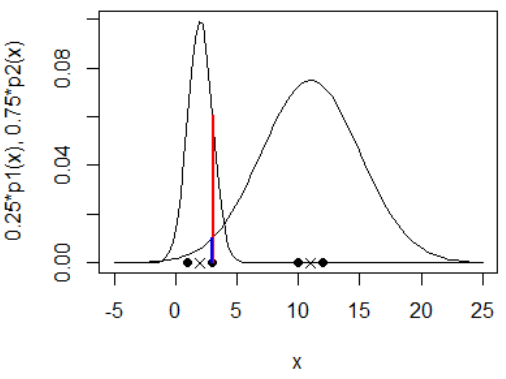
\includegraphics{screenshot006}
	\end{center}
		
	ne putem uita la cele două înălțimi colorate (roșu pentru $0.25 \cdot \mathcal{N}(3;2,1^2)$, albastru pentru $0.75 \cdot \mathcal{N}(3;11,4^2)$) și putem calcula rapoartele: 
	
	$P(Z_2 = 1|X_2= 3) = {\color{red}\dfrac{0.25\cdot \mathcal{N}(x_i;2,1^2)}{0.25\cdot \mathcal{N}(x_i;2,1^2) + {\color{blue}0.75\cdot\mathcal{N}(x;11,4^2)}}}$ și
	
	 $P(Z_2 = 2|X_2= 3) = {\color{blue}\dfrac{0.75\cdot \mathcal{N}(x_i;11,4^2)}{{\color{red}0.25\cdot \mathcal{N}(x_i;2,1^2)} + 0.75\cdot\mathcal{N}(x;11,4^2)}}$. 
	 
	 \textbf{Mai mult, dacă ne-ar interesa o clusterizare \textbf{hard} obținută din cea soft (luând maximul dintre $P(Z_2 = 1|X_2=3)$ și $P(Z_2 = 2|X_2=3)$), nu mai e nevoie să calculăm nimic, ci am asigna punctul 3 la clusterul corespunzător înălțimii mai mari, deci clusterului/gaussienei 1: $\color{red}\mathcal{N}(2,1^1)$.}
	
		\textbf{Observație 3}: Singura piesă lipsă este următoarea: Am început secțiunea \textit{Clusterizare via EM/GMM} cu date \textbf{și mixtura} ce a generat datele. Noi în realitate avem doar datele. Putem rezolva acest neajuns prin setarea unui număr $k$ de clustere/gaussiene. Apoi cu algoritmul EM/GMM învățăm parametrii mixturii. Astfel, avem și datele, și mixtura ce generează datele și putem clusteriza datele după cum tocmai am prezentat mai sus.
	\newpage
	\section{EM: Alte idei}
	
	Unele idei au fost preluate din sumarul capitolului \textit{Clusterizare} din carte (vezi pag. 466).
	
	\begin{itemize}
		\item În general, \textbf{schema algoritmică EM} este următoarea:
		\begin{algorithmic}
			\STATE Initialization: $\theta^{(0)}\gets$ initializeParameters(data)
			\FOR{t = 1:maxIterations} 
			\STATE $E$ step: compute $Q(\theta|\theta^{(t-1)})$
			\STATE $M$ step: $\theta^{(t)} = \arg \max_\theta Q(\theta|\theta^{(t-1)})$
			\ENDFOR
		\end{algorithmic}
		
		\item $Z_{ij} \equiv 1\{Z_i = j\}$; în multe locuri în carte/slide-uri nu apare $1\{Z_i = j\}$, ci $Z_{ij}$; trebuie să știți că ele înseamnă același lucru
		
		\item Trebuie să știți demonstrația de aici: \url{https://profs.info.uaic.ro/~ciortuz/SLIDES/cluster.pdf} slide-uri \#30-33. Este vorba de ex. 48 din carte. De fapt, aici este demonstrația de la Exercițiul 5a de mai sus lucrând cu date în general. (Dacă se face la curs, )Trebuie să știți și ex. 17 din carte unde se derivează alg. EM/GMM pentru orice date variind toți parametrii, nu doar $\mu$-urile, adică suntem în cazul Exercițiului 5b de mai sus.
		
		\item De ce merge EM, adică de ce maximizează funcția de verosimilitate a datelor observabile? Nu mai avem timp să vă spunem asta. Puteți citi voi (după sesiune) ex 1, 2 din Capitolul EM.
		
		\item În general, \textbf{se poate demonstra că $Q(\theta|\theta^{(t-1)})$ este o margine inferioară pentru funcția de log-verosimilitate a datelor observabile $l_D(\theta)$ (și de aceea are sens să o maximizăm).}
		
		\item Există o \textbf{similaritate între algoritmii k-means și EM/GMM}: vezi varianta de k-means de la ex. 39, unde există valorile $\gamma_{ij} \in \{0,1\}$ (hard...); în algoritmul EM/GMM avem $\gamma_{ij} \in [0,1]$ (soft...)!
		
		\item Există o \textbf{echivalență între algoritmii k-means și EM/GMM}: pentru detalii vezi ca idee ex. 54; esența: \textbf{dacă toate varianțele distribuțiilor normale sunt egale cu un $\sigma$ și tind spre 0 ($\sigma^2 \rightarrow 0$), atunci k-means $\equiv$ EM/GMM}; într-un caz oarecum opus, \textbf{când varianțele distribuțiilor normale sunt \textit{relativ} mari, apare un fenomen de \textbf{atracție reciprocă a mediilor}} gaussienelor (aceste medii fiind echivalentul centroizilor din algoritmul k-means), datorită faptului că fiecare instanță aparține cu o anumită probabilitate la fiecare cluster (vezi ex. 15b)
		
		\item Comparativ cu algoritmul k-means, algoritmul EM/GMM este în general mai lent - mișcarea centroizilor poate explora într-o manieră mai fină spațiul (vezi ex. 19).
		
		\item Rezultatele algoritmului EM depind (ca și la k-means) de valorile atribuite parametrilor la inițializare.
		
		\item \textbf{Inițializarea} contează: \textbf{nu inițializați toate $\mu$-urile la fel (și toate $\sigma$-urile la fel, dacă e cazul) pentru că algoritmul, după o iterație va ajunge la aceiași parametri}: vezi ex. 18
		
		\item Spre deosebire de cazul algoritmlui k-means, suprafețele / granițele de separare create de algoritmul EM/GMM nu sunt în mod neapărat liniare (vezi ex. 15c).
		
		\item Cam așa arată un grafic cu evoluția valorii funcției de log-verosimilitate calculată în parametrii găsiți la o anumită iterație:
		\begin{center}
			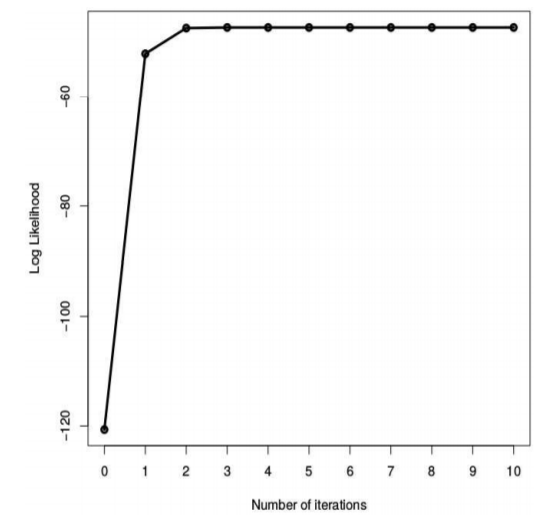
\includegraphics{screenshot005}
		\end{center}
		
		
		\item reiau cele două aplicații web menționate:
		\begin{itemize}
			\item pentru Bayes Naiv Gaussian unidimensional: \url{https://ml-fii.shinyapps.io/gnb_1d/}
			\item pentru EM/GMM unidimensional: \url{https://ml-fii.shinyapps.io/emApp/} (înainte să dați click pe \textit{Next Iteration}, încercați să vă imaginați cam pe unde se vor afla gaussienele la iterația următoare; verificați-vă intuiția apăsând pe \textit{Next Iteration})
		\end{itemize}
	\end{itemize}
	
	\newpage
	\textbf{\large{Schemă de final}}
	\begin{enumerate}
		\item Remember
		\begin{enumerate}
			\item Distribuții de probabilitate
			\item Mixturi de distribuții de probabilitate
			\item MLE
		\end{enumerate}
		\item Verosimilitate
		\item Log-verosimilitate
		\item Algoritmul EM
		\begin{enumerate}
			\item Algoritmul EM/GMM 
			\begin{enumerate}
				\item unde doar $\mu$-urile variază
				\item unde toți parametrii variază
			\end{enumerate}
		\end{enumerate}
	\end{enumerate}
	

	
\end{document}